%% LLT: Turn off some annoying warnings...
\RequirePackage{silence}
\WarningFilter{titlesec}{Non standard sectioning command}
\WarningFilter{scrreprt}{Usage of package}
\WarningFilter{scrreprt}{Activating an ugly workaround}
\RequirePackage[dvipsnames,table]{xcolor}
% *********************************************************
% CHOOSE THEME (ucph, sund, science, hum, samf, jura, teo)
% *********************************************************
\newcommand{\thesisTheme}{ucph} % to colortheme and titlepage image


% *********************************************************
% DOCUMENT CLASS
% *********************************************************
\documentclass[%
	paper=A4,					% paper size
	12pt,						% font size
	twoside=true,				% two-sided printing
	%openright,					% doublepage cleaning ends up right side
	openany,                    % chapters ends up on any side
	parskip=full,				% spacing value / method for paragraphs
	chapterprefix=true,			% prefix for chapter marks
	headings=normal,			% size of headings
	bibliography=totoc,			% include bib in toc
	listof=totoc,				% include listof entries in toc
	titlepage=on,				% own page for each title page
	captions=tableabove,		% display table captions above the float env
	draft=false,				% value for draft version
	abstract=on                 % abstract title on/off
]{scrreprt}
\usepackage[utf8]{inputenc}
\usepackage[english]{babel}
\usepackage{subcaption}
\usepackage{mathtools}
\usepackage{longtable}
\usepackage{physics}
\usepackage{amsmath}
\allowdisplaybreaks[1]
\numberwithin{equation}{chapter} % Change to select depth of equation numbering
\usepackage{placeins}% adjust the language
\usepackage{pdfpages}
\usepackage{pgfplots}
\usepackage{mathptmx}
\usepackage{paralist}
\usepackage{graphicx}
\usepackage{mathrsfs}
% \usepackage{epstopdf}
\usepackage{multirow}
\usepackage{listings}
\usepackage{tabularx}
% \usepackage{siunitx}
\usepackage{wrapfig}
\usepackage{lipsum}
\usepackage[format=plain]{caption}
\usepackage{array}
\usepackage{float}
\usepackage{tikz}
\usepackage{bm}
\usepackage[most]{tcolorbox}
% \usepackage[mathscr]{euscript}
\usepackage{amssymb}
\usepackage[extra]{tipa}

\raggedbottom
\captionsetup{singlelinecheck=false}
\pgfplotsset{compat=1.17}

% **************************************************
% COMMANDS FOR REUSE
% **************************************************

% Thesis
\newcommand{\thesisTitle}{Massively lockstep-parallel algorithms for full-isomer space quantum chemistry}
\newcommand{\thesisSubtitle}{}
\newcommand{\thesisName}{
  Anton M. Nielsen \& Asmus Tørsleff
}
\newcommand{\thesisSubject}{Masters} % May want to use (Bachelor, BSc, Masters or similar)
\newcommand{\thesisDate}{August 15, 2025}
\newcommand{\thesisVersion}{First Version}

% Supervisors & Collaborators
%\newcommand{\thesisExternalSupervisor}{}
\newcommand{\thesisInternalSupervisor}{
  Assoc. Professor, Ph.D. James Avery
}
\newcommand{\thesisInternalCoSupervisor}{
  Professor, Ph.D., Dr. Scient. Kurt V. Mikkelsen
}
\newcommand{\thesisCollab}{}

% University of Copenhagen
\newcommand{\thesisUniversity}{\protect{University of Copenhagen}}
\newcommand{\thesisFaculty}{Faculty of Science}
\newcommand{\thesisInstitute}{Department of Computer Science}
\newcommand{\thesisInstituteSecond}{Quantum Information Science}
\newcommand{\thesisCity}{Copenhagen {\O}}
\newcommand{\thesisAddress}{Universitetsparken 5}
\newcommand{\thesisPostal}{2100}

% *********************************************************
% PACKAGES
% *********************************************************

% OUR OWN PACKAGES!

\usepackage{amsmath}
\usepackage{braket}
\usepackage{dirtree}
\usepackage{hyperref}
\usepackage{minted}
\setminted{
  frame=single,
  framesep=5pt,
  breaklines,
  obeytabs=true,
  tabsize=4,
  linenos,
  numbersep=-12pt
}
\usepackage{tikz}
\usetikzlibrary{positioning}
\usetikzlibrary{fit}
\usetikzlibrary{calc}

%%


\usepackage[					% UCPH thesis style
    figuresep=colon,        
    sansserif=false,        
    hangfigurecaption=false,
    hangsection=true,       
    hangsubsection=true,
    hangsubsubsection=true, 
    colorize=full,          
    colortheme={\thesisTheme},  % ucph, sund, science, hum, etc.?
    bibsys=biber,
    bibfile=references,       % defines your .bib file
    bibstyle=numeric-comp,        % refer to https://bit.ly/2YsvIJz
]{ucphthesis}
\hypersetup{					% setup the hyperref-package options
	pdftitle={\thesisTitle},	% 	- title (PDF meta)
	pdfsubject={\thesisSubject},% 	- subject (PDF meta)
	pdfauthor={\thesisName},	% 	- author (PDF meta)
	plainpages=false,			% 	-
	colorlinks=false,			% 	- colorize links
	pdfborder={0 0 0},			% 	-
	breaklinks=true,			% 	- allow line break inside links
	bookmarksnumbered=true,		%
	bookmarksopen=true,			%
}

% *********************************************************
% Cover page content
% *********************************************************
%\subject{\vspace{3.0cm} \thesisSubject}
\subject{\vspace{2.5cm}}
\title{\thesisTitle}
\subtitle{\thesisSubtitle}
\author{\small{\thesisSubject} \\
        \thesisName \\
        \small{Supervised by {\thesisInternalSupervisor}}\\[-1.5ex]
        \small{Co-supervised by {\thesisInternalCoSupervisor}}\\
        \small{\thesisInstitute}\\[-1.5ex]
        \small{\thesisInstituteSecond}
    }
\date{\thesisDate}

% ********************************************************* 
% THESIS CONTENT
% *********************************************************



\DeclarePairedDelimiter\floor{\lfloor}{\rfloor}
\DeclarePairedDelimiter\ceil{\lceil}{\rceil}


\makeatletter
\newcommand\E{\@ifnextchar[{\@with}{\@without}}
\def\@with[#1]#2{E_{#2}^{(#1)}}
\def\@without#1{E_{#1}}
\makeatother

\makeatletter
\newcommand{\q}[1]{\textbf{QUESTION: #1}}
\makeatother

\newcommand\mn[1]{#1_{\mu\nu}}
\makeatletter
\newcommand\footnoteref[1]{\protected@xdef\@thefnmark{\ref{#1}}\@footnotemark}
\makeatother

\begin{document}

% -------------------------- 
% Front matter
% --------------------------
\pagenumbering{roman}
\pagestyle{empty}				            % no header or footers
\AddToShipoutPicture*{\TitleBackground}     % adding background picture
\maketitle                                  % making the title
% Cover back page
\AddToShipoutPicture*{\TitleWatermark}% adding watermark
\vspace{2.5cm}
{
    \begin{center}
	\small
	\textbf{\thesisSubject}\\
	\vspace{1.5cm}
	\large\textit{\thesisTitle} \\
	\vspace{1.5cm}
	\normalsize By \thesisName \\
	\vspace{1.5cm}
	Supervised by \thesisInternalSupervisor \\[-0.5ex]
	Co-supervised by \thesisInternalCoSupervisor \\[1.5em]
	Date of submission: \thesisDate \\
	\end{center}
	\vspace{5.0cm}
	\small
	\textbf{\thesisUniversity} \\
	\textit{\thesisFaculty} \\
	\thesisInstitute \\
  \thesisInstituteSecond \\
	\thesisAddress \\
	\thesisPostal\ \thesisCity
}

   % \clearpage

\pagestyle{plain}
\pdfbookmark[0]{Acknowledgements}{Acknowledgements}
\chapter*{Acknowledgements}
\label{chap:acknowl}

We would like to thank our supervisor James E. Avery for guidance and advise during this project, especially in recommending articles and frequently checking in on the project.

We would also like to thank our co-supervisor Kurt V. Mikkelsen sharing his encyclopedic chemistry expertise and for his expedient and intuitive introduction to the chemistry.

We would like to thanks Jonas D. de la Cour for technical help, answering questions and advocating for us in the first few meetings regarding the project.

\vspace*{\fill} 
\begin{quote} 
\centering 
"I would like to thank my family, friends, and colleagues for their support and for being understanding of my absence during the last few weeks of the project." - Anton
\end{quote}
\vspace*{2em}
\begin{quote} 
\centering 
"Thank you to my family, friends and especially room-mate for caring for and tolerating a very spent co-inhabitant in the final days before hand-in." - Asmus
\end{quote}
\vspace*{\fill}
\vspace*{\fill}

\pdfbookmark[0]{Abstract}{Abstract}
\chapter*{Abstract}
We take a step towards faster screening for large isomer spaces of fullerenes by introducing both GPU and quantum algorithms for approximating their chemical energies. To this end we implement a prototype for large parts of a semi-empirical method obtaining energies matching the reference implementation. We show that this method is lockstep-parallel for isomer spaces with fixed element ordering and how to reduce computations by only considering fullerenes. The quantum algorithms provided allow sampling of isomers with low isotropic energy from the entire isomer space, with better than classical probability, using qubits logarithmic in the size of the isomer space and having circuit depth quadratic in the number of atoms in an isomer. 
 
\pdfbookmark[0]{Individual Contributions to the Project}{Individual Contributions to the Project}
\chapter*{Individual Contributions to the Project}
Due to the type of thesis this is handed in as, we will disclose which sections are individual contributions and responsibilities of each author and which are common. Regardless, every section has been proof read and discussed in common. 

Anton has contributed and taken responsibility for section \ref{sec:hppc} and section \ref{sec:testing} as well as the related code, including the Nix setup.

Asmus has contributed and taken responsibility for section \ref{sec:quant} and any paragraph mentioning quantum computation.



    \clearpage

\renewcommand{\cfttoctitlefont}{\thesischapterfont}
\renewcommand{\cftchapfont}{\normalsize\bfseries}
\renewcommand{\contentsname}{Table of Contents}
\setcounter{tocdepth}{2}		% define depth of toc
\tableofcontents				% display table of contents
    \clearpage


% -------------------------- 
% Main matter
% --------------------------
\pagenumbering{arabic}			% arabic page numbering
\setcounter{page}{1}			% set page counter
\pagestyle{maincontentstyle} 	% fancy header and footer

%Inkluder flere Chapters her

\begin{refsection}

\part{Thesis}

\chapter{Introduction}
Calculating the properties of molecules is of major interest to any chemist. Computational approaches have become astonishingly precise and are of great use. A challenge is that the more accurate methods usually take weeks or months to run on large molecules. If we want results in a more timely manner we either have to spend more money on hardware, make faster software and algorithms or find a way to do more targeted calculations. 

In this thesis we will contribute to James E. Avery's efforts to develop an efficient screening pipeline for fullerenes. The concept of a screening pipeline applies when you want to calculate the properties of a large amount of molecules e.g. large isomer spaces in search of the best molecules for your purposes. In such a pipeline progressively slower techniques are used in each step while discarding poor candidate molecules in each. 

For our purpose we work with the isomer spaces $C_n$ where their size is on the order of $O(n^9)$.
These quickly become very large and so the first step in the screening pipeline must be very efficient. This motivates picking a fast approximate algorithm and implementing a highly optimised version.
We landed on GFN2-xTB for this role. It is part of a family of algorithms for computing the geometries, frequencies and noncovalent bonds using extended tight binding methods. It is semi-emperical and already decently fast. 

Calculating the properties of a molecule in $C_200$ takes about 30 seconds on a good desktop using the GFN2-xTB reference implementation. A quick back of the envelope calculation then puts the time to calculate all the molecules in the $C_200$ isomer space at around 200 years. To bring this down we now only have two levers to pull, acquiring more hardware or faster software. 

Thus this thesis will provide a blueprint for accelerating the calculation of entire isomer spaces of highly similar molecules in GFN2-xTB, as well as an in-depth look at the GFN2-xTB algorithm. We will exploit the fact that fullerenes are entirely made up of carbon atoms to provide lock-step parallel algorithms suitable for running on GPUs and taking advantage of their high floating point operation throughput.

We will also evaluate the opportunities for using quantum computing to speed up the search for good candidates. We will design quantum circuits for computing the GFN2-xTB isotropic energy terms and discuss how this can be applied to superposition's of molecules from an isomer space. 

In chapter \ref{sec:code_struct} we will introduce the repository structure, and in chapter \ref{sec:gfn2} we will explain the GFN2-xTB method including code snippets. In chapter \ref{sec:hppc} we will go over the practicalities of designing and implementing a lock-step parallel algorithm on the GPU. In chapter \ref{sec:quant} we will Design and analyse quantum circuits as an alternative approach to calculating the anisotropic energy terms of GFN2-xTB. In chapter \ref{sec:related} we will briefly discuss related projects. Chapter \ref{sec:meth} introduces our implementation approach and how we ensure correctness in relation to the reference implementation. In chapters \ref{sec:results}, \ref{sec:reflection} and \ref{sec:conclusion} we reflect on and conclude the project while reiterating our results.

\newpage
\chapter{Code Structure}\label{sec:code_struct}

The code repository can be found at: \url{https://github.com/AceMouse/xTB-math}.

\dirtree{%
.1 xTB-math/.
.2 bin2xyz/.
.3 bin2xyz.cpp\DTcomment{converter from float64 coords into xyz format}.
.3 C200\_10000\_fullerenes.float64\DTcomment{3d coords for 10k fullerenes}.
.2 flake.lock.
.2 flake.nix\DTcomment{conventional structure for Nix inputs and outputs}.
.2 nix/\DTcomment{Nix package definitions for xtb and its dependencies}.
.3 cpx.nix\DTcomment{CPCM-X - a solvation model}.
.3 numsa.nix\DTcomment{solvent accessible surface area calculation}.
.3 patches/\DTcomment{patches for extracting data for validation}.
.4 dftd4/\DTcomment{dispersion correction}.
.5 log\_args\_and\_outputs.patch.
.5 use\_gfn2.patch.
.4 xtb/.
.5 log\_args\_and\_outputs.patch.
.5 log\_electro.patch.
.5 log\_utils.patch.
.3 xtb.nix\DTcomment{extended tight-binding program}.
.2 README.md.
.2 report/.
.2 xtb-python/\DTcomment{Python port of xTB paper and Fortran impl}.
.3 basisset.py.
.3 blas.py.
.3 cmp\_impls.py\DTcomment{validation tests against Fortran impl}.
.3 data/.
.4 C200.xyz.
.4 caffeine.xyz.
.3 dftd4.py\DTcomment{computation for dispersion correction}.
.3 dftd4\_reference.py\DTcomment{constants for dftd4}.
.3 energy.py\DTcomment{various energy computations}.
.3 fock.py\DTcomment{Fock matrix computation}.
.3 gfn2.py\DTcomment{GFN2-xTB specific constants}.
.3 lapack.py\DTcomment{Facade for LAPACK functions}.
.3 scc.py\DTcomment{computation for self-consistent charges}.
.3 slater.py\DTcomment{computation for slater determinants}.
.3 util.py.
.3 xyz\_reader.py.
}

\newpage

A seperate code repository for the SYCL GPU implementation can be found at: \url{https://github.com/Maroka-chan/xtb-gpu}.
\dirtree{%
.1 xtb-gpu/.
.2 flake.lock.
.2 flake.nix.
.2 nix/.
.3 nvhpc.nix\DTcomment{patching nvhpc to make nvfortran work on Nix}.
.3 xtb.nix\DTcomment{xtb version 6.4.0 compiled with nvfortran}.
.2 README.md.
.2 sycl/.
.3 build\_SDQH0.cpp\DTcomment{incomplete SYCL impl for build\_SDQH0}.
.3 data\_caffeine/\DTcomment{test data for electro.cpp computed from caffeine}.
.4 atomicGam.txt.
.4 dqsh.txt.
.4 dq.txt.
.4 H0.txt.
.4 jmat.txt.
.4 P.txt.
.4 shellGam.txt.
.4 shift.txt.
.3 data\_c200/\DTcomment{test data for electro.cpp computed from a C200 fullerene}.
.4 atomicGam.txt.
.4 ....
.3 electro.cpp\DTcomment{SYCL impl for computing electrostatic energy}.
}


A staging repository for the code that ended up in this report can be found at \url{https://github.com/AceMouse/Simple-GFNn-xTB}
\dirtree{%
.1 Simple-GFNn-xTB/.
.2 chemistry\_constants.py\DTcomment{well known constants, not specific to any method}.
.2 cmp\_impls.py\DTcomment{validation tests against Fortran impl}.
.2 D4\_constants.py\DTcomment{constants referenced in D4'}.
.2 data/.
.2 file\_formats.py\DTcomment{for reading xyz and coord files}.
.2 flake.lock.
.2 flake.nix.
.2 GFN2\_constants.py\DTcomment{constants referenced in GFN2-xTB}.
.2 GFN2\_xTB.py\DTcomment{Implementation of GFN2-xTB}.
.2 README.md.
.2 slater\_constants.py\DTcomment{constants related the approximation of STOs in GFN2-xTB}.
}


\chapter{Theory}
\section{GFN2-xTB}
GFN2-xTB is a part of the GFNn-xTB (Geometry, Frequency, Non covalent, eXtended Tight Binding) family of semi-empirical methods for computational chemistry. 

The method gives good approximations for molecular geometries, vibrational frequencies, and non-covalent interaction energies and also does well on a variety other properties. 
Overall it strives to hit a balance between being accurate, close to the physics, general over a wide range of elements and not too computationally expensive.

This is achieved by approximating a true quantum mechanical simulation, using carefully chosen approximations and parameters. 
In contrast to forcefield methods that often operate on the level of atoms or even functional groups interacting, GFN2-xTB still treats the calculations at the level of individual orbitals in many places. 

GFN2-xTB uses a Self-Consistent Charges (SCC) approach i.e. it makes an initial guess at a density matrix and an energy which it then iteratively refines until both have converged. We are mostly interested in the final energy. 

\subsection{Energy terms}
The terms in GFN2-xTB that determine the energy are as follows
\begin{equation}
E =\E{rep}+\E{disp}^{D4'}+\E{EHT}+\E{\gamma}+\E{AES}+\E{AXC}+\E{\Gamma} + G_{Fermi}
\end{equation}

TODO: snak med Kurt om anisotropiske termer og fermi.

We then have to also factor in the SCC. 
Let us consider the following code sketch in figure \ref{lst:total_energy} which we will fill out in this chapter. The chapter will go over each term and add code snippets illustrating the mathematics in a more concrete way. 
\begin{figure}[H]
\begin{minted}{python}
def get_GFN2_energy(atoms: list[int], positions : list[list[float]]) -> float:
    density = density_initial_guess(atoms)
    overlap, dipol_dipol, charge_quadrupol = overlap(atoms, positions)
    initial_hamiltonian = H0(atoms, positions)
    huckel_theory_matrix = H_EHT(atoms, positions, overlap, initial_hamiltonian)
    charges = mulliken_population_analysis(density,atoms)
    eigen_values = diagonalize(initial_hamiltonian, overlap) # HC=SCe 
    E_repulsion = repulsion(atoms, positions)
    E_dispersion = D4Prime(charges, atoms, positions)
    E_huckel = Huckel(density, extended_huckel_theory_matrix)
    E_anisotropic = AES(charges, overlap, dipol_dipol, charge_quadrupol, positions)
    E_isotropic = IES(charges, positions)
    E_fermi = Fermi(...)
    E = E_repulsion + E_dispersion + E_huckel + E_anisotropic + E_isotropic + E_Fermi
    while not (energy_converged and densities_converged):
        # change densities along the gradients and 
        # update everything using the new density
        # ...
        energy_converged = (E-E_new)**2 < tolerance
        densities_converged = error_squared(density, new_density) < tolerance
        E = E_new
        density = new_density
\end{minted}
\caption{Python code illustrating the main loop of a GFN2-xTB implementation.
Line 2-16 computes the energy in a non SCC manner, line 15-23 iteratively improves the energy using SCC.
Another way to describe this is that the zeroth iteration of SCC happens outside the loop as there is some setup required. 
}
    \label{lst:total_energy}
\end{figure}
Let us define a small helper function to decrease the amount of indentation in the later code examples. This will allow us to easily loop over the orbitals and know which atom and shell each belongs to. 
\begin{figure}[H]
\begin{minted}{python}
def get_orbitals(atoms: list[int]) -> list[tuple[int]]:
    orbitals = []
    for atom_idx,atom in enumerate(atoms):
        for subshell in range(number_of_subshells[atom]):
            l = angular_momentum_of_subshell[atom][subshell] 
            for orbital in range(l*2+1):
                orbitals.append((atom_idx,atom,subshell,orbital))
    return orbitals
\end{minted}
\caption{Python code for generating a convenient list of orbitals to iterate though. }
\end{figure}

And some functions used when we want to signal to the reader that the python list we just created will stay a fixed size. Additionally we get to contain the python list comprehension syntax here. 

\begin{figure}[H]
\begin{minted}{python}
def vector(n: int) -> list[float]:
    return [0.0 for _ in range(n)]

def square_matrix(n: int) -> list[list[float]]:
    return [[0.0 for _ in range(n)] for _ in range(n)]

def square_matrix_of_vectors(n: int, v:int) -> list[list[list[float]]]:
    return [[[0.0 for _ in range(v)] for _ in range(n)] for _ in range(n)]
\end{minted}
    \caption{Python code for creating a $n$ long vector, $n\times n$ matrix and $n\times n \times v$ tensor.}
\end{figure}
\subsection{Constructing the initial density matrix}
Many of the terms use the density matrix as part of their calculation and it is central to the SCC method. In the GFN2 paper the initial density matrix guess is formulated as a superposition of neutral atomic reference densities $P_0 = \sum_{A}P_{A_0}$. In simpler terms this means that we let $P_0$ be a diagonal matrix that is $n$ by $n$ where $n$ is the total number of orbitals across the whole molecule. The values on the diagonal are the fractional number of electrons in the orbitals, the fractional occupations. They are reference densities so we get them in a table we can index into per subshell, thus we just have to divide the electrons evenly between the orbitals in the subshell. The number of orbitals in a subshell is $2l+1$ where l is the quantum number corresponding to the angular momentum of the subshell.
\begin{figure}[H]
\begin{minted}{python}
def density_initial_guess(atoms: list[int]) -> list[list[float]]:
    orbitals = get_orbitals(atoms)
    fractional_occupations = square_matrix(len(orbitals))
    for orbital_idx,(_,atom,subshell,_) in enumerate(orbitals):
        l = angular_momentum_of_subshell[atom][subshell] 
        orbitals_in_subshell = l*2+1 
        electrons_in_subshell = reference_occupations[atom][subshell]
        electrons_per_orbital = electrons_in_subshell/orbitals_in_subshell
        fractional_occupations[orbital_idx][orbital_idx] = electrons_per_orbital
    return fractional_occupations
\end{minted}
\caption{Python code for computation of the initial density matrix $P_0$}
    \label{lst:orbitals}
\end{figure}
For fullerenes the guess is simply all ones on the diagonal as \verb|number_of_subshells[C] = 2|, \verb|angular_momentum_of_subshell[C] = [0,1,0]| and \verb|reference_occupations[C] = [1.0,3.0,0.0]|.
Here \verb|C=5| is the index for carbon. 
Thus \verb|fractional_occupations| will contain a repeating series of $\frac{1}{0\cdot2+1},\frac{3}{1\cdot2+1},\frac{3}{1\cdot2+1},\frac{3}{1\cdot2+1}$ on the diagonal.

\subsection{Constructing the overlap, dipol and quadrupol tensors}
We need the overlap matrix, $S$, for several of the terms.
The related dipol and quadrupol tensors denoted $D$ and $Q$ are also needed and due to their very similar construction we will go over the implementation and mathematics in one fell swoop. 
An element in each tensor is computed in the following way.
\begin{align}
    S_{\nu\mu} &= \braket{\psi_\nu|\psi_\mu} &\forall \nu \in l \in A,\quad\forall\mu \in l' \in B, \\
    D_{\nu\mu}^{u} &= \braket{\psi_\nu|(r_u-{R_P}_u)|\psi_\mu}  &\forall  u\in x,y,z\\
    Q_{\nu\mu}^{uv} &= \braket{\psi_\nu|(r_u-{R_P}_u)(r_v-{R_P}_v)|\psi_\mu} &\forall  v\in x,y,z
\end{align}
These are integrals between two Slater type orbitals (STOs) over the positions $r$. When we write $l \in A$ we mean to iterate though the subshells in every element A and take their angular momentum. $\nu\in l$ means that we iterate though the $2l+1$ orbitals in the subshell with quantum number $m\in\{-l,..,0,..,l\}$. See figure \ref{lst:orbitals} for a code example. ${R_P}$ is the $x,y,z$ position of the product of the orbitals, we will define this later.

For $D$ there are 3 unique values, corresponding to the 3 dimensions, to compute for each pair of orbitals which we will pack into an array. 
Since $(r_u-{R_P}_u)(r_v-{R_P}_v)=(r_v-{R_P}_v)(r_u-{R_P}_u)$ there are 6, rather than 9, unique combinations of dimensions to compute for each element in the $Q$ tensor which we will also pack into an array.
For the sake of clarity we will define the indices corresponding to the combinations of directions, these are however arbitrary and only used for array indexing.  
\begin{figure}[H]
\begin{minted}{python}
    x = 0
    y = 1
    z = 2
    xx = 0
    yy = 1
    zz = 2
    xy = 3
    xz = 4
    yz = 5
\end{minted}
\caption{Constants for the combinations of directions.}
\end{figure}
\begin{figure}[H]
\begin{minted}{python}
    def overlap_dipol_quadrupol(atoms: list[int], positions: list[list[float]])-> tuple[list[list[float]],list[list[list[float]]],list[list[list[float]]]]:
    orbitals = get_orbitals(atoms)
    S = square_matrix(len(orbitals))
    D = square_matrix_of_vectors(len(orbitals),3)
    Q = square_matrix_of_vectors(len(orbitals),6)
    for idx_A, (atom_idx_A,atom_A,subshell_A,orbital_A) in enumerate(orbitals):
        for idx_B, (atom_idx_B,atom_B,subshell_B,orbital_B) in enumerate(orbitals):
            R_A = positions[atom_idx_A]
            R_B = positions[atom_idx_B]
            l_A = angular_momentum_of_subshell[atom_A][subshell_A]
            l_B = angular_momentum_of_subshell[atom_B][subshell_B]
            s,d,q = compute_STO_integrals(...)
            S[idx_A][idx_B] = s
            for dir in [x,y,z]:
                D[idx_A][idx_B][dir] = d[dir]
            for dir in [xx,yy,zz,xy,xz,yz]:
                Q[idx_A][idx_B][dir] = q[dir]
    return S,D,Q
\end{minted}
\caption{Python snippet illustrating construction of the overlap, dipol and quadrupol tensors; $S,D$ and $Q$.}
\end{figure}

To compute the integrals we need to remember that in GFN2-xTB an STO is approximated as a linear combination of gaussian type orbitals:
\begin{equation}
    \begin{split}
        \ket{\psi_\nu} =&\psi(\zeta_{A,l},r-R_A) \\
        = &N_{STO,l}|r-R_A|^{n-1}e^{-\zeta_{A,l}|r-R_A|}Y_l^m(r-R_A)\\
        \approx &\sum_i^{N_{A,l}}c_{i,\nu}N_{GTO,l}(r_x-{R_A}_x)^{l_x}(r_y-{R_A}_y)^{l_y}(r_z-{R_A}_z)^{l_z}e^{-\alpha_{i,\nu}|r-R_A|^2}\\
        =& \sum_i^{N_{A,l}}c_{i,\nu}\phi(\alpha_{i,\nu},r-R_A)\\
        =& \sum_i^{N_{A,l}}c_{i,\nu}\ket{\phi_i}
    \end{split}
\end{equation}
Where $N_{A,l}$ is an element and shell dependant constant, it is the number of GTOs used to approximate the STO. $\zeta$ and $\alpha$ are the slater and gaussian exponents. The contraction coefficient $c$ is a fitted value, it is fitted with the assumption that $\zeta=1$ and to get the value we will actually be using, we need to scale the fitted value by $\zeta^2$. $R_A$ is the position of atom $A$. $N_{STO,l}$ and $N_{GTO,l}$ are normalisation terms. 
We will refer to the terms $(r_u-{R_A}_u)^{l_u}\quad\forall{u\in x,y,z}$ as polynomial prefactors. 
The approximation in terms of GTOs means we can express our overlap in terms of GTO integrals instead:
\begin{align}
    S_{\nu\mu} &=\sum_i^{N_{A,l}}\sum_j^{N_{B,l'}}c_{i,\nu}c_{j,\mu} \braket{\phi_i|\phi_j}\\
    D_{\nu\mu}^u &=\sum_i^{N_{A,l}}\sum_j^{N_{B,l'}}c_{i,\nu}c_{j,\mu} \braket{\phi_i|(r_u-{R_P}_u)|\phi_j}\\
    Q_{\nu\mu}^{uv} &=\sum_i^{N_{A,l}}\sum_j^{N_{B,l'}}c_{i,\nu}c_{j,\mu} \braket{\phi_i|(r_u-{R_P}_u)(r_v-{R_P}_v)|\phi_j}
\end{align}
\begin{figure}[H]
\begin{minted}{python}
def compute_STO_integrals(...) -> tuple[float,list[float],list[float]]:
    number_of_gaussians_A = number_of_gaussians[atom_A][subshell_A]
    number_of_gaussians_B = number_of_gaussians[atom_B][subshell_B]
    slater_exponent_A = slater_exponents[atom_A][subshell_A]
    slater_exponent_B = slater_exponents[atom_B][subshell_B]
    overlap = 0
    dipol = vector(3)
    quadrupol = vector(6)
    for gaussian_i in range(number_of_gaussians_A):
        for gaussian_j in range(number_of_gaussians_B):
            exponent_i = normalised_gaussian_exponent(...)
            exponent_j = normalised_gaussian_exponent(...)
            contraction_i = normalised_contraction_coeficient(...)
            contraction_j = normalised_contraction_coeficient(...)
            s,d,q = compute_GTO_integrals(...)
            overlap += contraction_i*contraction_j*s
            for dir in [x,y,z]:
                dipol[dir] += contraction_i*contraction_j*d[dir]
            for dir in [xx,yy,zz,xy,xz,yz]:
                quadrupol[dir] += contraction_i*contraction_j*q[dir]
    return overlap,dipol,quadrupol
\end{minted}
    \caption{Python snippet illustrating construction of the STO integrals $\braket{\psi_\nu|\cdots|\psi_\mu}$.}
\end{figure}

For an s-orbital the normalisation terms would be:
\begin{align}
    N_{STO,0}&=\sqrt{\frac{\zeta_{A,l}^3}{\pi}}\\
    N_{GTO,0}&=\left(\frac{2\alpha_{i,\nu}}{\pi}\right)^{3/4}
\end{align}
TODO: snak med kurt om den generelle form.

We only need the GTO ones and can compute them in the following way:
\begin{figure}[H]
\begin{minted}{python}
def normalised_gaussian_exponent(atom:int, subshell:int, gaussian:int, slater_exponent:float) -> float:
    normalisation_factor = slater_exponent**2
    return gaussian_exponents[atom][subshell][gaussian]*normalisation_factor

def normalised_contraction_coefficient(atom:int, subshell:int, gaussian:int, gaussian_exponent:float) -> float:
    l = angular_momentum_of_subshell[atom][subshell]
    normalization_factor = (((2.0*gaussian_exponent)/pi)**(3/4)) * (sqrt(4*gaussian_exponent)**l) / sqrt(double_factorial(l))
    return contraction_coeficients[atom][shell][gaussian]*normalisation_factor

def double_factorial(n:int) -> int:
    if n <= 1:
        return 1
    return n*double_factorial(n-2)
\end{minted}
    \caption{Python snippet illustrating normalisation of the gaussian exponents and contraction coefficients.}
\end{figure}

As the GTOs in the integral are real valued functions we can drop the conjugation when we write them out.

For the overlap matrix:
\begin{align}
        \braket{\phi_i|\phi_j} = &\int \phi^*(\alpha_{i,\nu},r-R_A)\phi(\alpha_{j,\mu},r-R_B)\,dr\\
        =&\int \phi(\alpha_{i,\nu},r-R_A)\phi(\alpha_{j,\mu},r-R_B)\,dr\notag
\end{align}

For the dipol tensor:
\begin{align}
        \braket{\phi_i|(r_u-{R_P}_u)|\phi_j} = &\int \phi^*(\alpha_{i,\nu},r-R_A)(r_u-{R_P}_u)\phi(\alpha_{j,\mu},r-R_B)\,dr\\
        =&\int (r_u-{R_P}_u)\phi(\alpha_{i,\nu},r-R_A)\phi(\alpha_{j,\mu},r-R_B)\,dr\notag
\end{align}

For the quadrupol tensor:
\begin{align}
        \braket{\phi_i|(r_u-{R_P}_u)(r_v-{R_P}_v)|\phi_j} = &\int \phi^*(\alpha_{i,\nu},r-R_A)(r_u-{R_P}_u)(r_v-{R_P}_v)\phi(\alpha_{j,\mu},r-R_B)\,dr\\
        =&\int (r_u-{R_P}_u)(r_v-{R_P}_v)\phi(\alpha_{i,\nu},r-R_A)\phi(\alpha_{j,\mu},r-R_B)\,dr\notag
\end{align}
Now we see that we have to compute the products of GTOs. The product of two Gaussians is a new Gaussian centred at a point between the two, $R_P$, which we will finally introduce properly.
\begin{gather}
    \alpha = \alpha_{i,\nu}+\alpha_{j,\mu}\\
    K_{AB} = \left(\frac{2\alpha_{i,\nu}\alpha_{j,\mu}}{\alpha\pi}\right)^\frac{3}{4}e^{-\frac{\alpha_{i,\nu}\alpha_{j,\mu}}{\alpha}|R_A-R_B|^2}\\
    R_P = \frac{\alpha_{i,\nu}R_A+\alpha_{j,\mu}R_B}{\alpha}\\
    \phi(\alpha_{i,\mu},r-R_A)\phi(\alpha_{j,\nu},r-R_B) = K_{AB}\phi(\alpha,r-R_P)
\end{gather}
This rewrite only works if we also shift the polynomial prefactors to be relative to the product centre $R_P$, for all $u\in x,y,z$:
\begin{equation}
\begin{split}
    (r_u-{R_A}_u)^{{l_A}_u} = &\sum_{m_i=0}^{{l_A}_u}\binom{{l_A}_u}{m_i}({R_P}_u-{R_A}_u)^{({l_A}_u-m_i)}(r_u-{R_P}_u)^{{l_A}_u}\\
    =&\sum_{m_i=0}^{{l_A}_u}v_{m_i}(r_u-{R_P}_u)^{{l_A}_u}
\end{split}
\end{equation}
\begin{figure}[H]
\begin{minted}{python}
def shift_polynomial(l_dim, difference_to_P_dim) -> list[float]:
    poly_coefficients = vector(l_dim+1)
    for m in range(l_dim+1):
        poly_coefficients[m] = comb(l_dim, m)*difference_to_P_dim**(l_dim-m)
    return poly_coefficients
\end{minted}
    \caption{Python code illustrating computation of the shifted polynomial coefficients.}
\end{figure}
If we multiply these shifted prefactors we get the prefactors for the product. 
\begin{equation}
\begin{split}
    (r_u-{R_A}_u)^{{l_A}_u}(r_u-{R_B}_u)^{{l_B}_u} = &\sum_{m_i=0}^{{l_A}_u}\sum_{m_j=0}^{{l_B}_u}v_{m_i}v_{m_j}(r_u-{R_P}_u)^{{l_A}_u+{l_B}_u}\\
    =&\sum_t^{{l_A}_u+{l_B}_u}v_t(r_u-{R_P}_u)^t
\end{split}
\end{equation}

In the code we compute the values of $v_t$ as a convolution:
\begin{figure}[H]
\begin{minted}{python}
def convolute(coef_A, coef_B) -> float:
    max_t = len(coef_A)+len(coef_B)
    poly_coefficients = vector(max_t+1)
    for i,ci in enumerate(coef_A):
        for j,cj in enumerate(coef_B):
            poly_coefficients[i+j] += ci*cj
    return poly_coefficients
\end{minted}
    \caption{Python code illustrating computation of the $R_P$ polynomial coefficients via a convolution.}
\end{figure}


To compute the integrals over the GTOs we can split them in terms of the 3 dimensions we are integrating over, $x,y$ and $z$. We can also pull the GTO normalisation terms out front. 

For the overlap matrix:
\begin{align}
        \int \phi(\alpha_{i,\nu},r-R_A)\phi(\alpha_{j,\mu},r-R_B)\,dr=K_{AB}&\int \phi(\alpha,r-R_P)\,dr\\
        =N_{GTO,l_A}N_{GTO,l_B}K_{AB}&\int \phi(\alpha,r_x-{R_P}_x)\,dx\notag\\
            \times&\int \phi(\alpha,r_y-{R_P}_y)\,dy\notag\\
            \times&\int \phi(\alpha,r_z-{R_P}_z)\,dz\notag
\end{align}

For the dipol tensor:
\begin{align}
        \int (r_u-{R_P}_u)\phi(\alpha_{i,\nu},r-R_A)\phi(\alpha_{j,\mu},r-R_B)\,dr=K_{AB}&\int (r_u-{R_P}_u)\phi(\alpha,r-R_P)\,dr\\
        =N_{GTO,l_A}N_{GTO,l_B}K_{AB}&\int (r_u-{R_P}_u)\phi(\alpha,r_x-{R_P}_x)\,dx\notag\\
            \times&\int (r_u-{R_P}_u)\phi(\alpha,r_y-{R_P}_y)\,dy\notag\\
            \times&\int (r_u-{R_P}_u)\phi(\alpha,r_z-{R_P}_z)\,dz\notag
\end{align}

For the quadrupol tensor:
\begin{align}
        \int (r_u-{R_P}_u)(r_v-{R_P}_v)\phi(\alpha_{i,\nu},r-R_A)\phi(\alpha_{j,\mu},r-R_B)\,dr=K_{AB}&\int (r_u-{R_P}_u)(r_v-{R_P}_v)\phi(\alpha,r-R_P)\,dr\\
        =N_{GTO,l_A}N_{GTO,l_B}K_{AB}&\int (r_u-{R_P}_u)(r_v-{R_P}_v)\phi(\alpha,r_x-{R_P}_x)\,dx\notag\\
            \times&\int (r_u-{R_P}_u)(r_v-{R_P}_v)\phi(\alpha,r_y-{R_P}_y)\,dy\notag\\
            \times&\int (r_u-{R_P}_u)(r_v-{R_P}_v)\phi(\alpha,r_z-{R_P}_z)\,dz\notag
\end{align}
Each of these integrals can now be expanded using the analytical solution to Gaussian integrals of the form $\int x^t e^{-ax^2}\,dx$\cite{}. Let us briefly focus on the integrals over $x$ as they are all identical.

TODO: find den rigtig reference for eq 34 https://mathworld.wolfram.com/GaussianIntegral.html

For the overlap matrix:
\begin{align}
    \int \phi(\alpha,r_x-{R_P}_x)\,dx = \int \sum_{t=0}^{{l_A}_x+{l_B}_x}v_t(r_x-{R_P}_x)^te^{-\alpha|r_x-{R_P}_x|^2}\,dx\\
        =  \sum_{t=0}^{{l_A}_x+{l_B}_x}v_t\int(r_x-{R_P}_x)^{t}e^{-\alpha|r_x-{R_P}_x|^2}\,dx\notag\\
        =  \sum_{\{t\in0,..,{l_A}_x+{l_B}_x | odd(t)\}}v_{t}\frac{\left(\frac{t-1}{2}\right)!}{2a^{\frac{t+1}{2}}}+
        \sum_{\{t\in0,..,{l_A}_x+{l_B}_x | even(t)\}}v_{t}\frac{\left(t-1\right)!!}{2^{\frac{t}{2}+1}a^{\frac{t+1}{2}}}\sqrt{\frac{\pi}{\alpha}}\notag
\end{align}

For the dipol tensor:
\begin{align}
    \int (r_u-{R_P}_u)\phi(\alpha,r_x-{R_P}_x)\,dx = \int \sum_{t=0}^{{l_A}_x+{l_B}_x}v_t(r_u-{R_P}_u)(r_x-{R_P}_x)^te^{-\alpha|r_x-{R_P}_x|^2}\,dx\\
        =  \sum_{t=0}^{{l_A}_x+{l_B}_x}v_t\int(r_x-{R_P}_x)^{t+\delta_{ux}}e^{-\alpha|r_x-{R_P}_x|^2}\,dx\notag\\
        =  \sum_{t=\delta_{ux}}^{{l_A}_x+{l_B}_x+\delta_{ux}}v_{t-\delta_{ux}}\int(r_x-{R_P}_x)^{t}e^{-\alpha|r_x-{R_P}_x|^2}\,dx\notag\\
        =  \sum_{\{t\in\delta_{ux},..,{l_A}_x+{l_B}_x+\delta_{ux} | odd(t)\}}v_{t-\delta_{ux}}\frac{\left(\frac{t-1}{2}\right)!}{2a^{\frac{t+1}{2}}}+
        \sum_{\{t\in\delta_{ux},..,{l_A}_x+{l_B}_x+\delta_{ux} | even(t)\}}v_{t-\delta_{ux}}\frac{\left(t-1\right)!!}{2^{\frac{t}{2}+1}a^{\frac{t+1}{2}}}\sqrt{\frac{\pi}{\alpha}}\notag
\end{align}

For the quadrupol tensor:
\begin{align}
    \int (r_u-{R_P}_u)(r_v-{R_P}_v)\phi(\alpha,r_x-{R_P}_x)\,dx \\
    = \int \sum_{t=0}^{{l_A}_x+{l_B}_x}v_t(r_u-{R_P}_u)(r_v-{R_P}_v)(r_x-{R_P}_x)^te^{-\alpha|r_x-{R_P}_x|^2}\,dx\notag\\
        =  \sum_{t=0}^{{l_A}_x+{l_B}_x}v_t\int(r_x-{R_P}_x)^{t+\delta_{ux}+\delta_{vx}}e^{-\alpha|r_x-{R_P}_x|^2}\,dx\notag\\
        =  \sum_{t=\delta_{ux}+\delta_{vx}}^{{l_A}_x+{l_B}_x+\delta_{ux}}v_{t-\delta_{ux}-\delta_{-vx}}\int(r_x-{R_P}_x)^{t}e^{-\alpha|r_x-{R_P}_x|^2}\,dx\notag\\
        =  \sum_{\{t\in\delta_{ux}+\delta_{vx},..,{l_A}_x+{l_B}_x+\delta_{ux}+\delta_{vx} | odd(t)\}}v_{t-\delta_{ux}-\delta_{vx}}\frac{\left(\frac{t-1}{2}\right)!}{2a^{\frac{t+1}{2}}}+\notag\\
        \sum_{\{t\in\delta_{ux}+\delta_{vx},..,{l_A}_x+{l_B}_x+\delta_{ux}+\delta_{vx} | even(t)\}}v_{t-\delta_{ux}-\delta_{vx}}\frac{\left(t-1\right)!!}{2^{\frac{t}{2}+1}a^{\frac{t+1}{2}}}\sqrt{\frac{\pi}{\alpha}}\notag
\end{align}

TODO: Er det her rigtigt og i så fald hvor kommer $R_P^{(0,1,2)}$ termet i deres, og nu vores, kode fra?

The final sums are something we can compute. For the most part the analytical solution to the integrals is independent of the direction so we can precompute the independent part: 
\begin{figure}[H]
\begin{minted}{python}
def compute_gaussian_integral_factors(alpha:float, l_A:int, l_B:int)-> list[float]:
    factors = vector(l_A+l_B+3)
    for t in range(l_A+l_B+3):
        if t % 2 == 0:
            factors[t] = factorial((t-1)//2)/(2*alpha*((t+1)//2))
        else:
            factors[t] = (double_factorial(t-1)/(2**(t/2+1)*alpha**((t+1)//2))) * sqrt(pi/alpha)
    return factors
\end{minted}
    \caption{Python code illustrating computation of the integral factors for even and odd powers}
\end{figure}
We compute an extra $2$ factors to accommodate $\delta_{ux}+\delta_{vx}$

\begin{figure}[H]
\begin{minted}{python}
def compute_GTO_integrals(...)-> tuple[float,list[float],list[float]]:
    alpha = exponent_i + exponent_j
    exponents = exponent_i * exponent_j
    K_AB = ((2*exponents)/(alpha*pi))**(3/4) * e**(-(exponents/alpha)*distance)
    integral_factors = compute_gaussian_integral_factors(alpha, l_A, l_B)
    zeroth_moment = vector(3)
    first_moment = vector(3)
    second_moment = vector(3)
    for dim in [x,y,z]:
        gaussian_product_center_in_dim = (exponent_i*R_A[dim]+exponent_j*R_B[dim])/alpha
        centre_relative_to_A = gaussian_product_center_in_dim-R_A[dim]
        centre_relative_to_B = gaussian_product_center_in_dim-R_B[dim]
        l_A_dim = angular_momentum_in_dimension[l_A][orbital_A][dim]
        l_B_dim = angular_momentum_in_dimension[l_B][orbital_B][dim]
        l_max_dim = max(l_A_dim, l_B_dim)
        vmis = shift_polynomial(l_A_dim, centre_relative_to_A)
        vmjs = shift_polynomial(l_B_dim, centre_relative_to_B)
        vts = convolute(vmis, vmjs)
        for t, vt in enumerate(vts):
            zeroth_moment[dim] += vt * integral_factors[t+m]
            for m in range(1+1):
                first_moment[dim] += comb(1,m) * gaussian_product_center_in_dim**(1-m) * vt * integral_factors[t+m]
            for m in range(2+1):
                second_moment[dim] += comb(2,m) * gaussian_product_center_in_dim**(2-m) * vt * integral_factors[t+m]

    overlap = zeroth_moment[x]*zeroth_moment[y]*zeroth_moment[z]

    dipol = vector(3)
    dipol[x] = first_moment[x]*zeroth_moment[y]*zeroth_moment[z]
    dipol[y] = zeroth_moment[x]*first_moment[y]*zeroth_moment[z]
    dipol[z] = zeroth_moment[x]*zeroth_moment[y]*first_moment[z]

    quadrupol = vector(3)
    quadrupol[xx] = second_moment[x]*zeroth_moment[y]*zeroth_moment[z]
    quadrupol[yy] = zeroth_moment[x]*second_moment[y]*zeroth_moment[z]
    quadrupol[zz] = zeroth_moment[x]*zeroth_moment[y]*second_moment[z]
    quadrupol[xy] = first_moment[x]*first_moment[y]*zeroth_moment[z]
    quadrupol[xz] = first_moment[x]*zeroth_moment[y]*first_moment[z]
    quadrupol[yz] = zeroth_moment[x]*first_moment[y]*first_moment[z]
    return overlap, dipol, quadrupol
\end{minted}
    \caption{Python code illustrating computation of the integral $\braket{\phi_i|\cdots|\phi_j}$ using the dimension-wise decomposition.}
\end{figure}
%\begin{equation}
%N^{G}_{i}(\alpha_i,\ell_x,\ell_y,\ell_z)
%= \sqrt{\left(\frac{2\alpha_i}{\pi}\right)^{3/2}
%\frac{(4\alpha_i)^{\ell}}{(2\ell_x-1)!!\,(2\ell_y-1)!!\,(2\ell_z-1)!!}},
%\end{equation}

\subsection{Building the Hückel matrix}
As a part of computing the Hückel energy we need to construct the Hückel matrix.
The Hückel matrix comes from extended Hückel theory. Before we can construct it we need a few definitions. 
First the GFN2 type coordination number for atom $A$ is
\begin{gather}
    \begin{split}
        CN_A' = &\sum_{B\neq A}\left(1+e^{-10\left(\frac{4\left(R_{A,cov}+R_{B,cov}\right)}{3R_{AB}}-1\right)}\right)^{-1}\left(1+e^{-20\left(\frac{4\left(R_{A,cov}+R_{B,cov}+2\right)}{3R_{AB}}-1\right)}\right)^{-1}
    \end{split}
\end{gather}
Where $R_{A,cov}$ is the covalent atomic radius of $A$ specified for the GFN2 method. $R_{AB}$ is the euclidean distance between $A$ and $B$.
Now with $EN_A$ being the Pauling electronegativity and $k_EN=0.02$ as well as $k_{A,l}^{\text{poly}}$ being GFN2 specific constants we define the following 3 functions:
\begin{gather}
    X(EN_A,EN_B) = 1 + k_{EN}(EN_A-EN_B)^2\\
    \Pi(R_{AB},l,l') = \left(1 + k^{\text{poly}}_{A,l}\left(\frac{R_{AB}}{R_{A,cov}+R_{B,cov}}\right)^\frac{1}{2}\right)\left(1 + k^{\text{poly}}_{B,l'}\left(\frac{R_{AB}}{R_{A,cov}+R_{B,cov}}\right)^\frac{1}{2}\right)\\
    Y(\zeta_{A,l},\zeta_{B,l'}) = \left(\frac{2\sqrt{\zeta_{A,l}\zeta_{B,l'}}}{\zeta_{A,l}+\zeta_{B,l'}}\right)^\frac{1}{2}
\end{gather}

The Hückel matrix is then calculated as follows:
\begin{align}
    H_{\nu\nu}^{EHT} &= H_A^l - H_{CN_A}CN_A'\\
    \mn{H^{EHT}} &= \frac{1}{2}K^{ll'}_{AB}\mn{S}(H^{EHT}_{\mu\mu}+H^{EHT}_{\nu\nu})\\
    &\cdot X(EN_A,EN_B)\notag\\
    &\cdot \Pi(R_{AB},l,l')\notag\\
    &\cdot Y(\zeta^A_l,\zeta^B_{l'}), \quad\quad \forall \mu \in l \in A, \nu \in l' \in B\notag
\end{align}

$K^{ll'}_{AB}$ is an element and shell specific fitted constant however, in GFN2 it only depends on the shells. 
$S_{\mu\nu}=\braket{\phi_\mu|\phi_\nu}$ is the just introduced overlap of the orbitals. 
$H^l_A$ and $H^l_{CN'_A}$ are both fitted constants. $EN_A$ is the electronegativity of the element of atom A, given in the original \texttt{xtb} code. 

\begin{figure}[H]
\begin{minted}{python}
def huckel_matrix(atoms: list[int], positions: list[list[float]], overlap: list[list[float]]) -> list[list[float]]:
    orbitals = get_orbitals(atoms)
    H_EHT = square_matrix(len(orbitals))
    CN = get_coordination_numbers(atoms,positions)
    for orbital_idx, (atom_idx,atom,subshell,orbital) in enumerate(orbitals):
        CN_A = CN[atom_idx]
        H_A = self_energy[atom][subshell] # constant
        H_CN_A = GFN2_H_CN_A[atom][subshell] # constant
        H_EHT[orbital_idx][orbital_idx] = H_A - H_CN_A*CN_A

    for idx_A,(atom_A_idx,atom_A,subshell_A,_) in enumerate(orbitals):
        l_A = angular_momentum_of_subshell[atom_A][subshell_A]
        EN_A = electro_negativity[atom_A]
        R_A = positions[atom_A_idx]
        Rcov_A = covalent_radii[atom_A]
        k_poly_A = k_poly[atom_A][l_A]
        for idx_B,(atom_B_idx,atom_B,subshell_B,_) in enumerate(orbitals):
            if idx_A == idx_B:
                continue
            l_B = angular_momentum_of_subshell[atom_B][subshell_B]
            EN_B = electro_negativity[atom_B]
            R_B = positions[atom_B_idx]
            Rcov_B = covalent_radii[atom_B]
            k_poly_B = k_poly[atom_B][l_B]
            K_ll = GFN2_K_AB[l_A][l_B]
            delta_EN_squared = (EN_A-EN_B)**2
            k_EN = 0.02
            X = 1+k_EN*delta_EN_squared
            R_AB = euclidean_distance(R_A,R_B) 
            Rcov_AB = Rcov_A + Rcov_B 
            PI = (1+k_poly_A*sqrt(R_AB/Rcov_AB)) * (1+k_poly_B*sqrt(R_AB/Rcov_AB))
            slater_exp_A = slater_exponent[atom_A][l_A]
            slater_exp_B = slater_exponent[atom_B][l_B]
            Y = sqrt((2*sqrt(slater_exp_A*slater_exp_B)) / (slater_exp_A+slater_exp_B))
            H_nn = H_EHT[idx_A][idx_A]
            H_mm = H_EHT[idx_B][idx_B]
            S_nm = overlap[idx_B][idx_B]
            H_EHT[idx_A][idx_B] = k_ll*(1/2)*(H_nn+H_mm)*S_nm*Y*X*PI
    return H_EHT
\end{minted}
\caption{Python code illustrating construction of the Hückel matrix}
\end{figure}
Using this we can now compute the Hückel energy where $P$ is the density matrix at this point in the SCC procedure:
\begin{equation}
    \E{EHT} = \sum_{\mu\nu}P_{\mu\nu}H^{EHT}_{\mu\nu}\\
\end{equation}



\begin{figure}[H]
\begin{minted}{python}
def get_GFN2_Huckel_energy(density_matrix:list[list[int]], huckel_matrix:list[list[int]]) -> float:
    E_EHT = 0
    orbitals = len(density_matrix)
    for shell_mu in range(orbitals):
        for shell_nu in range(orbitals):
            E_EHT += density_matrix[shell_nu][shell_mu] * huckel_matrix[shell_mu][shell_nu]
    return E_EHT
\end{minted}
\caption{Python code illustrating computation of the Hückel energy}
\end{figure}


\subsection{Repulsion energy}
The repulsion energy in GFN2-xTB is computed classically using the following formula:
\begin{align}
    \E{rep} &= \frac{1}{2}\sum_{A}\sum_{B\neq A}\frac{Z^{eff}_A Z^{eff}_B}{R_{AB}}e^{-\sqrt{a_Aa_B}(R_{AB})^{(k_f)}}\\
k_f &= \begin{cases}1 & if A,B\in\{\text{H},\text{He}\}\\\frac{3}{2}&otherwise\end{cases} 
\end{align}
The effective nuclear charge $Z^{eff}$ and $a$ are variables fitted for each element. 
$R_{AB}$ is the distance between the A and B atoms.
This can be implemented in the following way:

\begin{figure}[H]
\begin{minted}{python}
H = 0
He = 1
def get_GFN2_repulsion_energy(atoms: list[int], positions : list[list[float]]) -> float:
    sum = 0
    for idx_A, (atom_A, position_A) in enumerate(zip(atoms, positions)):
        for idx_B, (atom_B, position_B) in enumerate(zip(atoms, positions)):
            if idx_A == idx_B:
                continue
            k_f = 3/2
            if atom_A in [H, He] and atom_B in [H, He]:
                k_f = 1
            R_AB = euclidean_distance(position_A, position_B)
            alpha_A = repulsion_alpha[atom_A]
            alpha_B = repulsion_alpha[atom_B]
            Y_A = effective_nuclear_charge[atom_A]
            Y_B = effective_nuclear_charge[atom_B]
            sum += ((Y_A*Y_B)/R_AB) * e ** ( - sqrt(alpha_A*alpha_B) * R_AB**k_f )
    E_rep = (1/2)*sum
    return E_rep
\end{minted}
\caption{Python code illustrating computation of the repulsion energy}
\end{figure}

\subsection{Isotropic Energy}
The isotropic energy terms $\E{\gamma}$ and $\E{\Gamma}$ require us to first do a Mulliken population analysis to get the subshell-wise partial Mulliken charges $q_{A,l}$.
\begin{equation}
    q_{A,l} = \text{TODO:Snak med kurt}\\
\end{equation}

With $\eta_A$ being an element specific constant and $k_{A,l}$ being a shell specific constant we define, both specific to the parametrisation of GFN2:
\begin{equation}
    \eta = \frac{(1+k_{A,l})\eta_A+(1+k_{B,l'})\eta_B}{2}\\
\end{equation}

\begin{equation}
    \gamma_{AB,ll'} = \sqrt{\frac{1}{R_{AB}^2+\eta^{-2}}}
\end{equation}
We can then define one of the two parts of the isotropic energy, $\E{\gamma}$
\begin{equation}
    \E{\gamma} = \frac{1}{2}\sum_{A,B}^{N_{atoms}}\sum_{l\in A}\sum_{l'\in B}q_{A,l}q_{B,l'}\gamma_{AB,ll'}
\end{equation}
With the element and shell specific GFN2 constant $\Gamma_{A,l}$ we also get the definition for the other part:
\begin{equation}
    \E{\Gamma} = \frac{1}{3}\sum_A^{N_{atoms}}\sum_{l\in A}(q_{A,l})^3\Gamma_{A,l}
\end{equation}



\section{High Performance Parallel Computing}

The xTB program uses a specified method of the GFN-xTB algorithm to compute various energies for a molecule. By default the program is set to use GFN2-xTB, which is also the method this project focuses on.

For a molecule on the smaller scale such as a caffeine molecule which has 24 atoms, the Fortran xTB program takes around $100$ms on a 12th gen intel mobile processor, while a fullerene with 200 carbon atoms takes about 23 seconds to compute. The computional time for even small molecules begins to be noticable, when the problem size grows to thousands or millions of molecules.

This project aims to compute the energies of fullerenes in the isomerspaces \(C_{20}, \cdots, C_{200} \). For isomerspaces of this scale, rather than improving the performance for individual molecules, what is truly interesting for this problem domain is speeding up largely concurrent xTB computations by running them in parallel on general purpose graphic processing units (GPGPUs).

The highest level of parallelization here is to compute all the energy terms of a molecule in the same kernel. There are no data dependencies between the computations of multiple molecules, and this makes it a perfect case for massive parallelization by distributing these isolated workloads across the thousands of threads supported on modern GPGPUs.
Within the area of computing, the idea of running the same operations in parallel is known as a lockstep system. With a focus on fullerenes, which consists exclusively of carbon atoms, this type of lockstep parallelization is exactly what we want to create, namely a fast and constant flow of data for the broader pipeline that this project is part of.

Since the executions of the xTB algorithm on each fullerene are completely isolated workloads, this means that the level of parallelization for a given isomer group, such as C20, scales with the amount of isomers in that group. This means that a much larger isomer group like C200 will also have a much greater level of parallelization.

The streaming multiprocessors (SMs) on a GPU are slower and simpler than the cores on a CPU. They have no branch prediction or other smart optimization techniques, but instead an SM has more threads it can execute in parallel in comparison to a CPU core which can only execute threads concurrently. The difference is that SMs can truly run its threads simultaniously, while CPU cores rely on context switching to make it seem like proccesses are running simultaniously. With SMs, working only on a few fullerenes will have a massive overhead from spinning up a kernel and copying data from the host(CPU) to the device(GPU), but the problem size for this project makes SMs a great fit.

The current Fortran implementation of the xTB program only takes a single molecule at a time, but when doing lockstep parallization it would be interesting to have an implementation that takes multiple molecules. This would avoid the overhead of starting multiple processes, and the program will have the data for all molecules, which gives opportunity for data coalescing by aligning the data as a structure of arrays (SOA) instead of an array of structures (AOS). It can also make copying data from the host to device more efficient since the data for multiple molecules can be moved together by the same instruction. To allow for coalesced access to the data on the device, we can essentially realign the data so that parts of the molecules that are accessed together, are also close together in memory.%Doing this should also decrease the amount of copies needed between host and device memory, resulting in overall faster execution.

\begin{figure}[h]
\centering
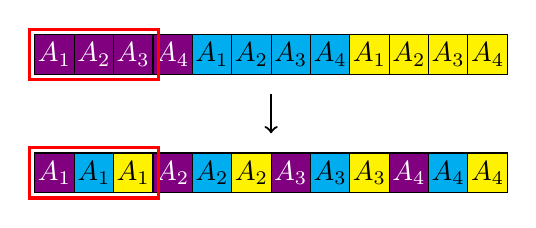
\begin{tikzpicture}[
squarednode/.style={
    rectangle,
    draw=black,
    fill=violet,
    text=white,
    thin,
    minimum size=5mm,
    inner sep=0pt, % No inner spacing
    outer sep=0pt, % No outer spacing
},
]

\node[squarednode] (A1) at (0,0) {$A_1$};
\node[squarednode, anchor=west] (A2) at (A1.east)   {$A_2$};
\node[squarednode, anchor=west] (A3) at (A2.east)   {$A_3$};
\node[squarednode, anchor=west] (A4) at (A3.east)   {$A_4$};

\node[squarednode, anchor=west, fill=cyan, text=black] (A1-2) at (A4.east)   {$A_1$};
\node[squarednode, anchor=west, fill=cyan, text=black] (A2-2) at (A1-2.east)   {$A_2$};
\node[squarednode, anchor=west, fill=cyan, text=black] (A3-2) at (A2-2.east)   {$A_3$};
\node[squarednode, anchor=west, fill=cyan, text=black] (A4-2) at (A3-2.east)   {$A_4$};

\node[squarednode, anchor=west, fill=yellow, text=black] (A1-3) at (A4-2.east)   {$A_1$};
\node[squarednode, anchor=west, fill=yellow, text=black] (A2-3) at (A1-3.east)   {$A_2$};
\node[squarednode, anchor=west, fill=yellow, text=black] (A3-3) at (A2-3.east)   {$A_3$};
\node[squarednode, anchor=west, fill=yellow, text=black] (A4-3) at (A3-3.east)   {$A_4$};



\node[squarednode, anchor=west] (A1-4) [below=of A1] {$A_1$};
\node[squarednode, anchor=west, fill=cyan, text=black] (A1-5) at (A1-4.east)   {$A_1$};
\node[squarednode, anchor=west, fill=yellow, text=black] (A1-6) at (A1-5.east)   {$A_1$};

\node[squarednode, anchor=west] (A2-4) at (A1-6.east)   {$A_2$};
\node[squarednode, anchor=west, fill=cyan, text=black] (A2-5) at (A2-4.east) {$A_2$};
\node[squarednode, anchor=west, fill=yellow, text=black] (A2-6) at (A2-5.east)   {$A_2$};

\node[squarednode, anchor=west] (A3-4) at (A2-6.east)   {$A_3$};
\node[squarednode, anchor=west, fill=cyan, text=black] (A3-5) at (A3-4.east)   {$A_3$};
\node[squarednode, anchor=west, fill=yellow, text=black] (A3-6) at (A3-5.east) {$A_3$};

\node[squarednode, anchor=west] (A4-4) at (A3-6.east)   {$A_4$};
\node[squarednode, anchor=west, fill=cyan, text=black] (A4-5) at (A4-4.east)   {$A_4$};
\node[squarednode, anchor=west, fill=yellow, text=black] (A4-6) at (A4-5.east)   {$A_4$};

\draw[->, thick] ($(A2-2.south) + (0.25,-0.25)$) -- ($(A2-6.north) + (0.25,0.25)$);

\node[draw=red, very thick, fit=(A1-4)(A1-5)(A1-6), inner sep=2pt] {};
\node[draw=red, very thick, fit=(A1)(A2)(A3), inner sep=2pt] {};

\end{tikzpicture}
\caption{Transforms arrays of structures where the memory for each structure is laid out contiguously, into a structure of arrays where data relevant for a computation is close together. This way of grouping related data close together is known as spatial locality and allows for coalesced access of the data.}
\label{fig:coalescing}
\end{figure}

An example of turning an AOS into an SOA can be seen in \autoref{fig:coalescing} where the data is realigned to allow for coalesced data access. If the code accesses only a few atoms of a molecule at a time, then it is a waste if the memory page contains the rest of a molecule as well. Instead of copying whole molecules at a time, the data should be structured such that only the required data of a molecule is copied as it allows the kernel to get that data for more molecules at a time, thus reducing unnecessary copies and speeding up the computation.

The geometric data for the fullerenes that are fed into the xTB implementation that our project focuses on, is already on the device and is never meant to leave the device before the final result is reached. The xTB implementation should therefore never move any data between the host and device. As such, memory coalescing is something to consider mainly when talking about the data transfer between the global and shared memory on a device. When we compute the energies for multiple molecules in the same SM, then we would like to move the necessary data for the current operation for all of the molecules in the SM together. The whole molecule will not fit in the lower memory levels, so we need to interweave the data of the molecules such that the necessary parts of the molecules can be moved together in as few operations as possible.

% Maybe find an example where we for example iterated through indices of two matrices such as the density and overlap matrices. In this case it could make sense to interweave them such that the indices accessed in iteration 1 is together and so on.

% We want to keep all data on the GPU, so we don't received in on the CPU, it is already on the GPU.
% Maybe explain how data coalescing makes sense when moving data between memoery levels on a GPU?


\subsection{Memory Types and Current Hardware}

The types of memory typically found in the memory hiearchy on a GPU are global, shared, local, and register memory. Using these levels of memory properly is crucial for achieving high performance in parallel computing tasks. Here is an overview of the various levels:

\begin{itemize}
  \item Global - Accessible from all threads on the GPU. This is the largest but also the slowest pool of memory.
  \item Shared - Tied to a thread block (or workgroup), so it can be accessed by the threads in the same thread block. This pool of memory is smaller but faster than global memory.
  \item Register Memory - Each thread on a GPU has private access to a number of registers. This is the fastest type of memory used to store local variables and intermediate results.
  \item Local Memory - Also private to each thread. This type is slower than register memory and is usually used when there is insufficient space for variables on the registers of a thread.
\end{itemize}


The NVIDIA Ada Lovelace GPU architecture\cite{nvidia-ada-tuning-guide} has $80$ GB of global memory, $100$ KB of shared memory per SM, and $64,000$ $32$-bit registers per SM, which gives us $256$ KB of register memory per SM.

\begin{equation}
\begin{split}
  64000 \cdot 32 &= 2048000 \text{ bits}\\
  &= 256000 \text{ bytes}\\
  &= 256 \text{ KB}
\end{split}
\end{equation}

Each thread has a maximum of $255$ registers, and each SM has a maximum of $24$ blocks and a maximum of $48$ warps. This adds up such that full utilization can be achieved when each block has $2$ warps allocated. A warp has $32$ threads, so an SM has a total of $1536$ threads when each of its $24$ blocks has two warps.
Distributing the $64,000$ registers evenly over these threads gives each of them $41$ registers, which is considerably lower than the maximum of $255$, but allows all of the threads to be used evenly. By using \autoref{eq:reg_mem_utilized_per_sm} we can see that this configuration utilizes $251.9$ KB of the register memory available to each of the SMs.

\begin{equation}
\begin{split}
  WarpsPerBlock &= \floor*{\frac{WarpsPerSM}{BlocksPerSM}}
\end{split}
\end{equation}

\begin{equation}
\begin{split}
  ThreadsPerBlock &= WarpsPerBlock \times ThreadsPerWarp
\end{split}
\end{equation}

\begin{equation}
\begin{split}
  RegistersPerThread &= \floor*{\frac{RegistersPerSM}{BlocksPerSM \times ThreadsPerBlock}}
\end{split}
\end{equation}

\begin{equation} \label{eq:reg_mem_utilized_per_sm}
\begin{split}
  RegisterMemoryUtilizedPerSM =\\
  &BlocksPerSM\\
  &\times ThreadsPerBlock\\
  &\times RegistersPerThread\\
  &\times BitsPerRegister
\end{split}
\end{equation}

BlocksPerSM and BitsPerRegister are constants found in the specification for the GPU architecture.

With this, each block in an SM has $10.496$ KB of register memory to work with, and thus each thread has $164$ bytes.

\begin{equation}
\begin{split}
  \frac{251.904}{24} &= 10.496 \text{ KB}
\end{split}
\end{equation}

\begin{equation}
\begin{split}
  \frac{251904}{1536} &= 164 \text{ bytes}
\end{split}
\end{equation}

The shared memory capacity per SM is $100$ KB and a single block can have a maximum of $99$ KB. This gives each block about $4.16$ KB of shared memory, meaning that the $64$ threads in a block will have $65$ bytes each.

\begin{equation}
\begin{split}
  \frac{100}{24} &= 4.166 \text{ KB}
\end{split}
\end{equation}

\begin{equation}
\begin{split}
  \frac{4166}{64} &= 65.09 \text{ bytes}
\end{split}
\end{equation}

The Ada Lovelace architecture has a total of $128$ SMs and it also has a $98304$ KB L2 cache. This results in a total of $3072$ blocks that each has $32$ KB of the L2 Cache. All of this combined gives each block a total of $46.656$ KB of non-global memory.

\begin{equation}
\begin{split}
  10.496 \text{ KB} + 4.166 \text{ KB} + 32 \text{ KB} &= 46.662 \text{ KB}
\end{split}
\end{equation}

Distributing the global memory across the blocks gives each of them $26.042$ MB. Combined with the non-global memory, this results in each block having a total of $26.088$ MB of memory.

\subsection{Optimizing GPU Configuration for Isolated Molecules}

Computing xTB-GFN2 for a molecule is completely isolated, so if we do the whole xTB computation in lockstep, then we only have to concern ourselves with how many warps and blocks a single molecule needs in order to keep all its data in device memory. When we know these details, then we can simply scale up the number of molecules to be computed in lockstep until all the resources on the GPU are saturated. With this approach, expanding to multiple GPUs should be rather trivial as there are no interdependencies.

The exact space needed to compute the GFN2 method of xTB for a single fullerene is not yet clear to us, and it will also vary based on the size of the fullerene. To make finding the most optimal GPU configuration easier when optimizing for most possible parallel xTB computations, we have developed a script that computes such a configuration based on the space requirement of a single molecule.

\begin{figure}[h!]
\begin{minted}{python}
  def compute(bytes_per_molecule):
    mb_per_molecule = bytes_per_molecule / 1_000_000

    threads_per_molecule = compute_threads_per_molecule(mb_per_molecule)
    warps_per_molecule = compute_warps_per_molecule(threads_per_molecule)
    molecules_per_block = compute_molecules_per_block(warps_per_molecule)

    print_utilization(warps_per_molecule, molecules_per_block)

    print(f"MB per molecule: {mb_per_molecule} MB")
    print(f"Threads per molecule: {threads_per_molecule}")
    print(f"Warps per molecule: {warps_per_molecule}")
    print(f"Molecules per block: {molecules_per_block}")
\end{minted}
  \caption{This is the top-level function for computing the optimal number of warps needed per molecule when optimizing for most possible parallel xTB computations on a single GPU specifically for the Ada Lovelace architecture.}
\end{figure}

The output of the script has information on how many threads are required for a single molecule, how many warps this fits within. It also includes general information about the utilization of the GPUs resources with the configuration presented. An example of the full output can be seen in \autoref{fig:gpu-mem-output}.


\begin{figure}[h!]
\begin{minted}[linenos=false]{text}
| Global memory | L2 cache | Total SMs | Threads per warp |
|    80.0 GB    | 98304 KB |    128    |        32        |
| Threads Available | Threads Used | Blocks Available | Blocks Used |
|      196608       |    196608    |       3072       |    3072.0   |

#################################### Per SM ####################################
| Warps | Blocks | Registers | Shared Memory | Threads Available | Threads Used |
|  48   |   24   |   64000   |    100 KB     |       1536        |     1536     |
| Blocks Available | Blocks Used |
|        24        |     24.0    |

########################### Per Block ###########################
| L2 Cache | Register Mem | Shared Mem | Global Mem | Total mem |
| 32.0 KB  |  10.496 KB   |  4.167 KB  |  26.042 MB | 26.088 MB |

MB per molecule: 8.3 MB
Threads per molecule: 18
Warps per molecule: 1
Molecules per block: 2
\end{minted}
\caption{This is the output of our script for computing an optimal GPU configuration when a single molecule needs $8.3$ MB of memory.}
\label{fig:gpu-mem-output}
\end{figure}

In \autoref{fig:gpu-mem-output} each molecule is $8.3$ MB and thus requires the memory of $18$ threads. Each warp has $32$ threads, so in this case a single molecule fits within a single warp. With $24$ blocks and $48$ warps per SM, all blocks can have $2$ warps each, which in this scenario means that $2$ molecules can be computed in parallel within a single block. This space requirement for a molecule is just an example and in no way guaranteed to be representative of the actual requirements of fullerenes of any size.


%The electrostatic energy term depends on the initial Huckel energy term H0, P, dq, dqsh, atomicGam, shellGam, jmat\_flat, shift...
%
%Instead of giving a bad approximation then just explain the equations and how to use the script.
%
%83GB for 10000 C200
%8.3 MB for each molecule
%SMs has max 48 warps
%each warp has 32 threads
%64000 32bit registers per SM
%each thread can max use 255 registers
%max thread blocks per SM is 24
%two thread blocks to make use of all 48 warps
%shared memory capacity per SM 100KB
%maximum shared memory per thread block is 99KB
%SMs schedule warps/workgroups/thread blocks
%we can do ~1536 molecules per SM with this amount of data




%Doing more fine grained parallelization can make use of SIMT(Single instruction multiple threads) like reduction.

\section{Introduction to quantum algorithmic approaches}
In this section we will attempt to construct quantum algorithms for calculating three of the GFN2-xTB\cite{bannwarth2019} energy terms: $E^\Gamma, E^\gamma$ and $E^{EHT}$.
We will showcase three different approaches to doing a calculation as a building block of a larger circuit.


The conceptually simplest approach is to directly translate classical mathematical circuits to the quantum world using ancillary qubits to ensure reversibility.
Here most of the computation happens in the state, and the result is readable in the bits of the measurement output.
This approach has seen some development beyond this simple translation resulting in some very qubit efficient primitives for multiplication and addition in particular\cite{draper2000,perez2017}.
This approach will be applied to the $E^\Gamma$ and $E^\gamma$ terms, and be referred to as Quantum Digital Arithmetic in this report. 


Our second approach is Quantum Amplitude Arithmetic\cite{wang2020}. 
In this approach we try to prepare the desired result not as a easily read measurement result, but as part of the amplitude of a state.
We will use this approach for the $E^\Gamma$ term to prepare a qubit in the state $w\ket{0}+\alpha\ket{0}$ where we can choose $\alpha$ to be proportional to the $E^\Gamma$ of the molecule.
Alternatively we can choose $\alpha$ to be proportional to $E^\Gamma-E^\Gamma_H$ where $E^\Gamma_H$ is the $E^\Gamma$ energy for some known high energy isomer.
This is not something we imagine being a common thing to want, however it is something which we want for the total energy! The issue that is solved by subtracting a known high energy is the following.
Say we know all the energies, and we want to do something with those states that have a low energy.
If all the energies lie between 100 and 101 (units not important), which may make a large difference, the relative difference is not large.
If we subtract a known high energy of say 100.9 we get much larger relative differences where the low energy isomers will have a much larger $\alpha$ than the high energy isomers. 


The final algorithmic approach we will explore uses quantum singular value transformations\cite{gilyen2019}.
In this approach the calculations are being carried out in the singular values of block encoded matrices. 
We will use this approach to calculate the $E^{ETH}$ term, as it involves a lot of elementwise matrix multiplications. 
This is well suited for this approach.


For all of these approaches we will assume that we have access to some pretty intricately prepared states. 
We will not go into how the are prepared other than the fact that classically we can generate the geometries and so for entire isomer spaces without any other information. 
As any classical computation in theory also can be applied to a quantum computer after modifications it is a possibility to prepare these states. 


\subsection{Calculating $E^\Gamma$ using Quantum Digital Arithmetic}
The GFN2-xTB $E^\Gamma$ term has the following form\cite{bannwarth2021}
\begin{equation}
    E^\Gamma = \frac{1}{3}\sum_A\sum_{\mu\in A} (q_{A,\mu})^3\Gamma_{A,\mu},
\end{equation}
where $q_{A,\nu}=\sum_B\sum_{\nu\in B}P_{\mu\nu}S_{\mu\nu}$ is the partial charge of shell $\mu$ associated with atom $A$. $P, S$ are the density and overlap matrices. $\Gamma_{A,\mu} = \Gamma_A K_\mu$ is just the product of an element specific constant and a shell specific constant, for our purposes the element is always carbon and the shell is either the first or second in GFN2 thus we have 2 numbers $\Gamma_{\text{Carbon},0(1)}$ henceforth referred to as $\varGamma_{0(1)}$. 

\vspace{\baselineskip}
\noindent
Let us first rewrite the inner expression a bit given our new definition and knowledge of the atoms we are working with. 
\begin{equation}
    \sum_{\mu\in A} (q_{A,\mu})^3\Gamma_{A,\mu} = \sum_{\mu \in \{0,1\}} (q_{A,\mu})^3\varGamma_{\mu}
\end{equation}

We now need a unitary which computes this function on a given state $\ket{\varGamma_\mu}_\Gamma\ket{q_{A,\mu}}_Q\ket{acc}_E \to \ket{\varGamma_\mu}_\Gamma\ket{q_{A,\mu}}_Q\ket{acc+(q_{A,\mu})^3\varGamma_{\mu}}_E$. The subscripts on the kets refer to the quantum register they represent. 
Consider having access to the following fused multiply add unitary $\ket{A}\ket{B}\ket{acc} \to \ket{A}\ket{B}\ket{acc+A*B}$. 
Let us to our initial $\Gamma, Q, E$ registers add two ancillary registers, $W_1,W_2$. 
We can now apply the following unitary 
\begin{equation}
    \resizebox{.9\hsize}{!}{${E_i^\Gamma}_{(\Gamma,Q,W_1,W_2,E)} = \text{MADD}^\dagger_{\Gamma,Q,W_1}\text{MADD}^\dagger_{Q,W_1,W_2}\text{MADD}_{Q,W_2,E}\text{MADD}_{Q,W_1,W_2}\text{MADD}_{\Gamma,Q,W_1}$}
    \label{EiG}
\end{equation}
\begin{figure}[H]
    \centering
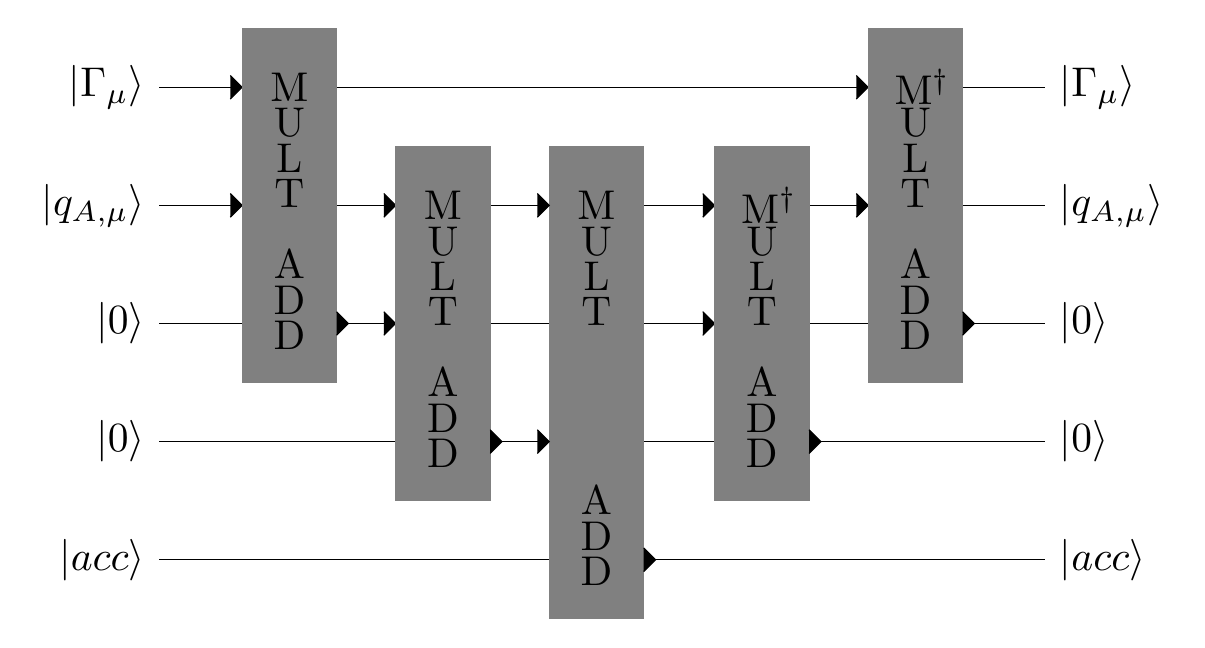
\begin{tikzpicture}[scale=1.5, transform shape]
    \node[rectangle,anchor=east] at (-1.5,4) {$\ket{\Gamma_\mu}$};
    \node[rectangle,anchor=east] at (-1.5,3) {$\ket{q_{A,\mu}}$};
    \node[rectangle,anchor=east] at (-1.5,2) {$\ket{0}$};
    \node[rectangle,anchor=east] at (-1.5,1) {$\ket{0}$};
    \node[rectangle,anchor=east] at (-1.5,0) {$\ket{acc}$};

    \node[rectangle,anchor=west] at ( 6,4) {$\ket{\Gamma_\mu}$};
    \node[rectangle,anchor=west] at ( 6,3) {$\ket{q_{A,\mu}}$};
    \node[rectangle,anchor=west] at ( 6,2) {$\ket{0}$};
    \node[rectangle,anchor=west] at ( 6,1) {$\ket{0}$};
    \node[rectangle,anchor=west] at ( 6,0) {$\ket{acc}$};
    \foreach \y in {0,...,4}
        \draw (-1.5,\y) -- (6,\y) ;
    \foreach \x in {0,...,1}{
        \filldraw[black] (\x*1.3-.9,2.9-\x) -- (\x*1.3-.8,3-\x) -- (\x*1.3-.9,3.1-\x);
        \filldraw[black] (\x*1.3-.9,3.9-\x) -- (\x*1.3-.8,4-\x) -- (\x*1.3-.9,4.1-\x);
        \filldraw[gray] (-0.8+\x*1.3+0,2-\x+2.5) rectangle (0+\x*1.3,1-\x+.5);
        \filldraw[black] (0+\x*1.3,1-\x+.9) -- (0+\x*1.3+0.1,1-\x+1) -- (0+\x*1.3,1-\x+1.1);
        \node[] at (-0.4+\x*1.3+0,2-\x+2.0) {M}; 
        \node[] at (-0.4+\x*1.3+0,2-\x+1.7) {U}; 
        \node[] at (-0.4+\x*1.3+0,2-\x+1.4) {L}; 
        \node[] at (-0.4+\x*1.3+0,2-\x+1.1) {T}; 
        \node[] at (-0.4+\x*1.3+0,2-\x+.5) {A}; 
        \node[] at (-0.4+\x*1.3+0,2-\x+.2) {D}; 
        \node[] at (-0.4+\x*1.3+0,2-\x-.1) {D}; 
    }
    \filldraw[gray] (-0.8+2*1.3+0,2-1+2.5) rectangle (0+2*1.3,1-2+.5);
    \filldraw[black] (0+2*1.3,1-2+.9) -- (0+2*1.3+0.1,1-2+1) -- (0+2*1.3,1-2+1.1);

    \filldraw[black] (2*1.3-.9,.9) -- (2*1.3-.8,1) -- (0+2*1.3-.9,1.1);
    \filldraw[black] (2*1.3-.9,2.9) -- (2*1.3-.8,3) -- (0+2*1.3-.9,3.1);
    \node[] at (-0.4+2*1.3+0,1+2.0) {M}; 
    \node[] at (-0.4+2*1.3+0,1+1.7) {U}; 
    \node[] at (-0.4+2*1.3+0,1+1.4) {L}; 
    \node[] at (-0.4+2*1.3+0,1+1.1) {T}; 
    \node[] at (-0.4+2*1.3+0,+.5) {A}; 
    \node[] at (-0.4+2*1.3+0,+.2) {D}; 
    \node[] at (-0.4+2*1.3+0,-.1) {D}; 
    \foreach \x in {0,...,1}{
        \filldraw[black] (4+\x*1.3-.9,2.9+\x) -- (4+\x*1.3-.8,3+\x) -- (4+\x*1.3-.9,3.1+\x);
        \filldraw[black] (4+\x*1.3-.9,1.9+\x) -- (4+\x*1.3-.8,2+\x) -- (4+\x*1.3-.9,2.1+\x);
        \filldraw[gray] (4+-0.8+\x*1.3+0,1+\x+2.5) rectangle (4+0+\x*1.3,+\x+.5);
        \filldraw[black] (4+0+\x*1.3,+\x+.9) -- (4+0+\x*1.3+0.1,+\x+1) -- (4+0+\x*1.3,+\x+1.1);
        \node[anchor=west] at (-0.4+\x*1.3+4-.3,1+\x+2.0) {M$ ^\dagger$}; 
        \node[] at (-0.4+\x*1.3+4,1+\x+1.7) {U}; 
        \node[] at (-0.4+\x*1.3+4,1+\x+1.4) {L}; 
        \node[] at (-0.4+\x*1.3+4,1+\x+1.1) {T}; 
        \node[] at (-0.4+\x*1.3+4,1+\x+.5) {A}; 
        \node[] at (-0.4+\x*1.3+4,1+\x+.2) {D}; 
        \node[] at (-0.4+\x*1.3+4,1+\x-.1) {D}; 
    }
\end{tikzpicture}
    \caption{Circuit implementing equation \ref{EiG}}
\end{figure}
Let us follow the process:

\begin{align}
    &{E_i^\Gamma}_{(\Gamma,Q,W_1,W_2,E)}\ket{\varGamma_\mu}_\Gamma\ket{q_{A,\mu}}_Q\ket{0}_{W_1}\ket{0}_{W_2}\ket{acc}_E\\
    =&\resizebox{.9\hsize}{!}{$\text{MADD}^\dagger_{\Gamma,Q,W_1}\text{MADD}^\dagger_{Q,W_1,W_2}\text{MADD}_{Q,W_2,E}\text{MADD}_{Q,W_1,W_2}\ket{\varGamma_\mu}_\Gamma\ket{q_{A,\mu}}_Q\ket{\varGamma_\mu q_{A,\mu}}_{W_1}\ket{0}_{W_2}\ket{acc}_E$}\\
    =&\resizebox{.9\hsize}{!}{$\text{MADD}^\dagger_{\Gamma,Q,W_1}\text{MADD}^\dagger_{Q,W_1,W_2}\text{MADD}_{Q,W_2,E}\ket{\varGamma_\mu}_\Gamma\ket{q_{A,\mu}}_Q\ket{\varGamma_\mu q_{A,\mu}}_{W_1}\ket{\varGamma_\mu (q_{A,\mu})^2}_{W_2}\ket{acc}_E$}\\
    =&\resizebox{.9\hsize}{!}{$\text{MADD}^\dagger_{\Gamma,Q,W_1}\text{MADD}^\dagger_{Q,W_1,W_2}\ket{\varGamma_\mu}_\Gamma\ket{q_{A,\mu}}_Q\ket{\varGamma_\mu q_{A,\mu}}_{W_1}\ket{\varGamma_\mu (q_{A,\mu})^2}_{W_2}\ket{acc+\varGamma_\mu (q_{A,\mu})^3}_E\label{comp}$}\\
    =&\text{MADD}^\dagger_{\Gamma,Q,W_1}\ket{\varGamma_\mu}_\Gamma\ket{q_{A,\mu}}_Q\ket{\varGamma_\mu q_{A,\mu}}_{W_1}\ket{0}_{W_2}\ket{acc+\varGamma_\mu (q_{A,\mu})^3}_E\\
    =&\ket{\varGamma_\mu}_\Gamma\ket{q_{A,\mu}}_Q\ket{0}_{W_1}\ket{0}_{W_2}\ket{acc+\varGamma_\mu (q_{A,\mu})^3}_E\\
\end{align}
We see that already in eq. \ref{comp} we have the result we want in the accumulation register. We continue with the uncomputation of the $W_1,W_2$ registers purely to be able to reuse them in the remaining calculations. This saves the qubits required for having a 2 ancillary registers for every calculation. The MADD gates here could be implementing using QFT multipliers\cite{perez2017} in which case we wouldn't need any additional ancillaries. If we decompose our QFT multiplier into its components it is essentially a chain of QFT additions\cite{draper2000,perez2017} and multiplications by a constant power of two. These additions are built up of two components: (inverse) Fourier transforms and conditional rotations. When we chain them together like this however many of the transforms can be taken out as they are always followed or preceded by their inverse except for in the beginning and end. 



Let us say we are given a circuit, SDA, for encoding a molecule from its ID in the following manner, and a circuit $\text{DA}=\prod_{A}\prod_{\mu\in \{0,1\}} {E_i^\Gamma}_{(\Gamma_\mu,Q_{A,\mu},W_1,W_2,E)}$. Then 
\begin{equation}
\begin{split}
    \text{DA}\ \text{SDA}&\ket{ID}_{ID}\ket{0}\to\\
    \text{DA}&\ket{ID}_{ID}\bigg(\bigotimes_{\mu\in \{0,1\}}\ket{\varGamma_\mu}_{\Gamma_\mu}\bigotimes_{A}\ket{q_{A,\mu}}_{Q_{A,\mu}}\bigg)\ket{0}_{W_1}\ket{0}_{W_2}\ket{0}_E \to\\
    &\ket{ID}_{ID}\bigg(\bigotimes_{\mu\in \{0,1\}}\ket{\varGamma_\mu}_{\Gamma_\mu}\bigotimes_{A}\ket{q_{A,\mu}}_{Q_{A,\mu}}\bigg)\ket{0}_{W_1}\ket{0}_{W_2}\ket{E^\Gamma}_E\\
\end{split}
\end{equation}
\noindent
will give us the $E^\Gamma$ energy term in the E register corresponding to the ID in the ID register.

\subsection{Sampling using Quantum Amplitude Arithmetic}
Assume that we are given an equal superposition of all the canonical IDs of the fullerenes in an isomer-space. We can apply SDA to set up the encoding and then apply $DA$. We now have computed the $E^\Gamma$ energies for every isomer. However we can only sample once! Let us say that we are interested in the isomers with the lowest energies. We then would like the probability of sampling an isomer to be proportional to $E^\Gamma$. We can achieve this using Quantum Amplitude Arithmetic\cite{wang2020}, not to be confused with Quantum Amplitude Amplification, both shortened as QAA but in this writing as QA-Arithmetic and QA-Amplification. 


\vspace{\baselineskip}
Wang et al. use their introduced addition and multiplication primitives to construct a circuit which transforms the state $\ket{x}_D\ket{0}_C\ket{0}_W \to \frac{1}{2}\frac{x}{2^n}\ket{x}_D\ket{0}_C\ket{1}_W+\alpha\ket{\omega}_{D \otimes C\otimes W}$ where $\alpha$ is some normalization factor, and $\ket{\omega}$ is some state with no overlap with the state containing all 0's in the control register, $C$, and 1 in the work register, $W$.


\vspace{\baselineskip}
When using this circuit we can treat the $E$ register containing our resulting $E^\Gamma$ term as the data register, $D$. We can reuse the $W_1,W_2$ registers as the control and work registers. Let us take a look at that.
\begin{equation}
   \resizebox{.9\hsize}{!}{$\begin{split}
       \sum_{ID\in \text{isomers}}&\ket{ID}_{ID}\bigg(\bigotimes_{\mu\in \{0,1\}}\ket{\varGamma_\mu}_{\Gamma_\mu}\bigotimes_{A}\ket{q_{A,\mu}}_{Q_{A,\mu}}\bigg)\ket{0}_{W_1}\ket{0}_{W_2}\ket{E^\Gamma}_E \to\\ 
       \sum_{ID\in \text{isomers}}&\ket{ID}_{ID}\bigg(\bigotimes_{\mu\in \{0,1\}}\ket{\varGamma_\mu}_{\Gamma_\mu}\bigotimes_{A}\ket{q_{A,\mu}}_{Q_{A,\mu}}\bigg)\left(\frac{1}{2}\frac{E^\Gamma_{ID}}{2^n}\ket{0}_{W_1}\ket{1}_{W_2}\ket{E^\Gamma_{ID}}_E+\alpha_{ID}\ket{\omega_{ID}}\right) \\ 
   \end{split}$}
\end{equation}
If we now sample from this superposition and postselect for $W_1 = 0$ and $W_2 = 1$ we are more likely to sample a low energy fullerene. The likelihood of sampling a given canonical fullerene ID is proportional with $E^\Gamma$ for that fullerene.



\subsection{Calculating $E^\Gamma$ with Quantum Amplitude Arithmetic.}
An alternative strategy would be to go all in on QA-Arithmetic and do all the arithmetic in the amplitudes. 
Here we would encode a molecule as follows
\begin{equation}
   \resizebox{.9\hsize}{!}{$\begin{split}
       \text{SAA}&\ket{ID}_{ID}\ket{0}_{E,E_w,C_E,q_{o(1,2,3)},\Gamma_w,\Gamma_{1,\dots,n},q_{1,\dots,n},C_{1,\dots,\lceil log(n+1) \rceil}}\\
       =&\ket{ID}_{ID}\ket{0}_{E,E_w,C_E,q_{o(1,2,3)},\Gamma_w}\bigotimes_{\mu\in\{0,1\}}\ket{\varGamma_\mu}_{\Gamma_{1,\dots,n}}\bigotimes_{A}\ket{q_{A,\mu}}_{q_{1,\dots,n}}\ket{0}_{C_{1,\dots,\lceil log(n+1) \rceil}}
   \end{split}$}
\end{equation}

Let us apply the following example circuit to our encoding. Here we focus on one pair of $q$ and $\Gamma$. 
\begin{figure}[H]
    \centering
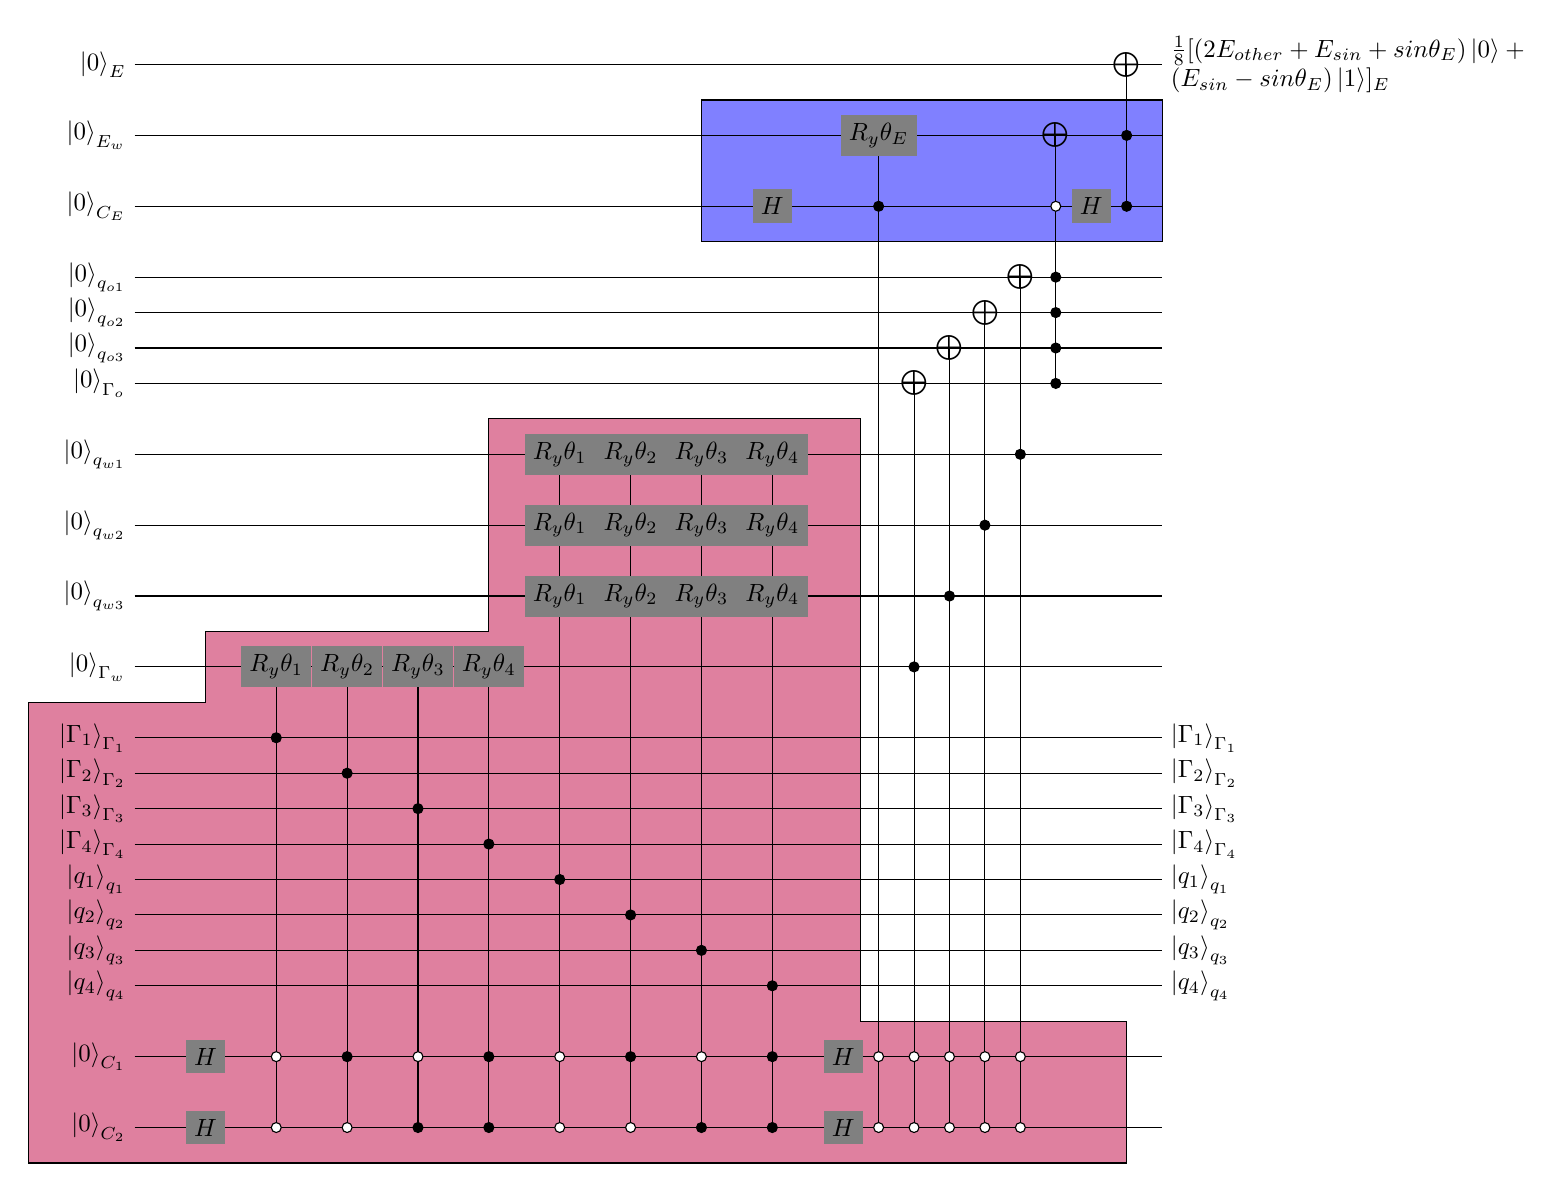
\begin{tikzpicture}[scale=0.9, transform shape]
    \draw[fill=purple!50] (-2.5,-.5) -- (-2.5,6) -- (0,6) -- (0,7) -- (4,7) -- (4,10) -- (9.25,10) -- (9.25,1.5) -- (13,1.5) -- (13,-.5) -- cycle;
    \draw[fill=blue!50] (7,12.5) -- (7,14.5) -- (13.5,14.5) -- (13.5,12.5) -- cycle;
    \foreach \y in {1,...,3}{
        \node[rectangle,anchor=east] at (-1,12.5-0.5*\y) {$\ket{0}_{q_{o\y}}$};
        \node[rectangle,anchor=east] at (-1,10.5-\y) { $\ket{0}_{q_{w\y}}$};
    }
    \node[rectangle,anchor=east] at (-1,10.5) {$\ket{0}_{\Gamma_o}$};
    \node[rectangle,anchor=east] at (-1,6.5) { $\ket{0}_{\Gamma_{w}}$};

    \node[text width=5cm,anchor=west] at (13.5,15) { $\frac{1}{8}[(2E_{other}+E_{sin}+sin\theta_E)\ket{0}+(E_{sin}-sin\theta_E)\ket{1}]_{E}$};


    \foreach \y in {1,...,4}
        \node[rectangle,anchor=east] at (-1,6-.5*\y) { $\ket{\Gamma_{\y}}_{\Gamma_{\y}}$};
    \foreach \y in {1,...,4}
        \node[rectangle,anchor=east] at (-1,4-.5*\y) { $\ket{q_{\y}}_{q_{\y}}$};
    \foreach \y in {1,2}
        \node[rectangle,anchor=east] at (-1,2-\y) { $\ket{0}_{C_{\y}}$};
    \node[rectangle,anchor=east] at (-1,13) { $\ket{0}_{C_E}$};
    \node[rectangle,anchor=east] at (-1,14) { $\ket{0}_{E_w}$};
    \node[rectangle,anchor=east] at (-1,15) { $\ket{0}_{E}$};

    \foreach \y in {1,...,4}
        \node[rectangle,anchor=west] at (13.5,6-.5*\y) { $\ket{\Gamma_{\y}}_{\Gamma_{\y}}$};
    \foreach \y in {1,...,4}
        \node[rectangle,anchor=west] at (13.5,4-.5*\y) { $\ket{q_{\y}}_{q_{\y}}$};

    \foreach \y in {0,...,2}
        \draw (-1,\y) -- (13.5,\y) ;
    \foreach \y in {3,...,9}
        \draw (-1,1+.5*\y) -- (13.5,1+.5*\y) ;
    \foreach \y in {1,...,3}
        \draw (-1,10.5+0.5*\y) -- (13.5,10.5+0.5*\y) ;
    \foreach \y in {1,...,3}
        \draw (-1,12+\y) -- (13.5,12+\y) ;
    \foreach \y in {10,...,14}
        \draw (-1,\y-3.5) -- (13.5,\y-3.5) ;
    \foreach \x in {1,...,4}{
        \draw (\x,0) -- (\x,6.5);
        \draw (\x+4,0) -- (\x+4,9.5);
    }
    \node[rectangle,fill=gray] at (0,0) {$H$} ;
    \node[rectangle,fill=gray] at (0,1) {$H$} ;
    \node[rectangle,fill=gray] at (9,0) {$H$} ;
    \node[rectangle,fill=gray] at (9,1) {$H$} ;
    \node[rectangle,fill=gray] at (8,13) {$H$} ;
    \node[rectangle,fill=gray] at (12.5,13) {$H$} ;
    \foreach \x in {1,...,4}{
        \node[rectangle,fill=gray] at (\x,6.5) {$R_y\theta_\x$} ;
        \foreach \y in {7.5,...,9.5}{
            \node[rectangle,fill=gray] at (\x+4,\y) {$R_y\theta_\x$} ;
        }
    }
    \draw (9.5,0) -- (9.5,14);
    \node[rectangle,fill=gray] at (9.5,14) {$R_y\theta_E$} ;
    \filldraw[black] (9.5,13) circle (2pt);
    \filldraw[white,draw=black] (9.5,0) circle (2pt);
    \filldraw[white,draw=black] (9.5,1) circle (2pt);

    \node[rectangle] at (12,14) {$\bigoplus$};
    \draw (12,10.5) -- (12,14);
    \foreach \y in {0,...,3}{
        \filldraw[black] (12,10.5+.5*\y) circle (2pt);
    }
    \filldraw[white,draw=black] (12,13) circle (2pt);
    \draw (13,13) -- (13,15);
    \node[rectangle] at (13,15) {$\bigoplus$};
    \filldraw[black] (13,13) circle (2pt);
    \filldraw[black] (13,14) circle (2pt);
    \foreach \a in {8,...,1}{
        \filldraw[black] (\a,6-0.5*\a) circle (2pt);
    }
    \foreach \g in {0,...,3}{
        \draw (10+0.5*\g,0) -- (10+0.5*\g,10.5+0.5*\g);
        \filldraw[white,draw=black] (10+0.5*\g,0) circle (2pt);
        \filldraw[white,draw=black] (10+0.5*\g,1) circle (2pt);
        \node[rectangle] at (0.5*\g+10,0.5*\g+10.5) {$\bigoplus$};
        \filldraw[black] (0.5*\g+10,\g+6.5) circle (2pt);
    }
    \foreach \x in {0,4}{
        \filldraw[black] (\x+2,1) circle (2pt);
        \filldraw[black] (\x+3,0) circle (2pt);
        \filldraw[black] (\x+4,1) circle (2pt);
        \filldraw[black] (\x+4,0) circle (2pt);
    }
    \foreach \x in {0,4}{
        \filldraw[white,draw=black] (\x+2,0) circle (2pt);
        \filldraw[white,draw=black] (\x+3,1) circle (2pt);
        \filldraw[white,draw=black] (\x+1,0) circle (2pt);
        \filldraw[white,draw=black] (\x+1,1) circle (2pt);
    }
\end{tikzpicture}
\caption{Circuit for computing $E^\Gamma-E^\Gamma_H$ on a one atom molecule where the charge $q$ and $\Gamma$ are described using 4 bytes. The crimson shaded area scales with the number of bits. The blue shaded area is for subtracting $E^\Gamma_H$ and is completely optional. }
\end{figure}
This circuit is built from the addition and multiplication primitives introduced in the QA-Arithmetic paper\cite{wang2020}. We also do a trivial modification to get subtraction. The diagram is for a n=4 bit example i.e. $q$ and $\Gamma$ are encoded as 4 bit numbers. The crimson region in the diagram is the only part which needs to be scaled up if using larger n. 

If using more than one $q$ and $\Gamma$ the contribution to the final $E_w$ register should include those as well which would just need an extra addition. $C_E$ should be scaled appropriately as the base 2 logarithm of the number of $q,\Gamma$ pairs plus 1.   

Let us go though the mathematics of our 4 bit example. 

The controlled gate notation here is the following, $t$ is the target register and $c1,c2,c3,\dots$ are the control registers. $a,b,c,\dots$ are all $1$ except if there is a bar over the corresponding $c1,c2,c3,\dots$ in which case it is $0$. 
\begin{equation}
    \begin{split}
        CU^{c1,c2,c3,\dots}_t = (U_t-I_t)\otimes &\ket{a}\bra{a}_{c1} \otimes \ket{b}\bra{b}_{c2} \otimes \ket{c}\bra{c}_{c3}\otimes\dots+\\ 
        \sum_{\alpha,\beta,\zeta,\dots\in\{0,1\}}I_t\otimes &\ket{\alpha}\bra{\alpha}_{c1} \otimes \ket{\beta}\bra{\beta}_{c2} \otimes \ket{\zeta}\bra{\zeta}_{c3}\otimes\dots. 
    \end{split}
\end{equation}
We neglect writing out the $q_{1,2,3,4},\Gamma_{1,2,3,4}$ as they never change throughout the calculation, we also neglect the registers outside of the crimson region for now. 
We begin by applying the Hadamard gates.
\begin{equation}
    \begin{split}
        H_{C1}H_{C2}&\ket{0000}_{q_{w(1,2,3)},\Gamma_w}\ket{ 00}_{C_{(1,2)}}\to\\
        \frac{1}{2}(
        &\ket{0000}_{q_{w(1,2,3)},\Gamma_w}\ket{ 00}_{C_{(1,2)}}+\\
        &\ket{0000}_{q_{w(1,2,3)},\Gamma_w}\ket{ 01}_{C_{(1,2)}}+\\
        &\ket{0000}_{q_{w(1,2,3)},\Gamma_w}\ket{ 10}_{C_{(1,2)}}+\\
        &\ket{0000}_{q_{w(1,2,3)},\Gamma_w}\ket{ 11}_{C_{(1,2)}}
        )
    \end{split}
\end{equation}
when we apply the conditional rotation gates to a register such as $\Gamma_w$ we do the following
\begin{equation}
   \resizebox{.9\hsize}{!}{$\begin{split}
        CRy_{\Gamma_w}^{\Gamma_4,C_1,C_2}(2\theta_4)CRy_{\Gamma_w}^{\Gamma_3,\bar{C_1},C_2}(2\theta_3)CRy_{\Gamma_w}^{\Gamma_2,C_1,\bar{C_2}}(2\theta_2)&CRy_{\Gamma_w}^{\Gamma_1,\bar{C_1},\bar{C_2}}(2\theta_1)\\
        \frac{1}{2}\sum_{x_1,x_2\in\{0,1\}}\ket{0000}_{q_{w(1,2,3)},\Gamma_w}&\ket{ x_1x_2}_{C_{(1,2)}}\to\\
        \frac{1}{2}(
        CRy_{\Gamma_w}^{\Gamma_1}(2\theta_1)\ket{0000}_{q_{w(1,2,3)},\Gamma_w}&\ket{ 00}_{C_{(1,2)}}+\\
        CRy_{\Gamma_w}^{\Gamma_2}(2\theta_2)\ket{0000}_{q_{w(1,2,3)},\Gamma_w}&\ket{ 01}_{C_{(1,2)}}+\\
        CRy_{\Gamma_w}^{\Gamma_3}(2\theta_3)\ket{0000}_{q_{w(1,2,3)},\Gamma_w}&\ket{ 10}_{C_{(1,2)}}+\\
        CRy_{\Gamma_w}^{\Gamma_4}(2\theta_4)\ket{0000}_{q_{w(1,2,3)},\Gamma_w}&\ket{ 11}_{C_{(1,2)}})\to\\
        \frac{1}{2}(
        \ket{000}[\Gamma1(cos\theta_1\ket{0}+sin\theta_1\ket{1})+(1-\Gamma_1)\ket{0}]_{q_{w(1,2,3)},\Gamma_w}&\ket{ 00}+\\
        \ket{000}[\Gamma2(cos\theta_2\ket{0}+sin\theta_2\ket{1})+(1-\Gamma_2)\ket{0}]_{q_{w(1,2,3)},\Gamma_w}&\ket{ 01}+\\
        \ket{000}[\Gamma3(cos\theta_3\ket{0}+sin\theta_3\ket{1})+(1-\Gamma_3)\ket{0}]_{q_{w(1,2,3)},\Gamma_w}&\ket{ 10}+\\
        \ket{000}[\Gamma4(cos\theta_4\ket{0}+sin\theta_4\ket{1})+(1-\Gamma_4)\ket{0}]_{q_{w(1,2,3)},\Gamma_w}&\ket{ 11}
        )
   \end{split}$}
\end{equation}
Let us adopt the notation $\ket{\Psi^t_i}=t(cos\theta_i\ket{0}+sin\theta_i\ket{1})+(1-t)\ket{0}$ before redoing the application using our new notation. We also apply the rotation gates for the $q_w$ registers:
\begin{equation}
   \resizebox{.9\hsize}{!}{$\begin{split}
        CRy_{\Gamma_w}^{\Gamma_4,C_1,C_2}(2\theta_4)CRy_{\Gamma_w}^{\Gamma_3,\bar{C_1},C_2}(2\theta_3)CRy_{\Gamma_w}^{\Gamma_2,C_1,\bar{C_2}}(2\theta_2)&CRy_{\Gamma_w}^{\Gamma_1,\bar{C_1},\bar{C_2}}(2\theta_1)\\
        CRy_{q_{w1}}^{q_4,C_1,C_2}(2\theta_4)CRy_{q_{w1}}^{q_3,\bar{C_1},C_2}(2\theta_3)CRy_{q_{w1}}^{q_2,C_1,\bar{C_2}}(2\theta_2)&CRy_{q_{w1}}^{q_1,\bar{C_1},\bar{C_2}}(2\theta_1)\\
        CRy_{q_{w2}}^{q_4,C_1,C_2}(2\theta_4)CRy_{q_{w2}}^{q_3,\bar{C_1},C_2}(2\theta_3)CRy_{q_{w2}}^{q_2,C_1,\bar{C_2}}(2\theta_2)&CRy_{q_{w2}}^{q_1,\bar{C_1},\bar{C_2}}(2\theta_1)\\
        CRy_{q_{w3}}^{q_4,C_1,C_2}(2\theta_4)CRy_{q_{w3}}^{q_3,\bar{C_1},C_2}(2\theta_3)CRy_{q_{w3}}^{q_2,C_1,\bar{C_2}}(2\theta_2)&CRy_{q_{w3}}^{q_1,\bar{C_1},\bar{C_2}}(2\theta_1)\\
        \frac{1}{2}\sum_{x_1,x_2\in\{0,1\}}\ket{0000}_{q_{w(1,2,3)},\Gamma_w}&\ket{ x_1x_2}=\\
        \frac{1}{2}(
        CRy_{q_{w1}}^{q_1}(2\theta_1)CRy_{q_{w2}}^{q_1}(2\theta_1)CRy_{q_{w3}}^{q_1}(2\theta_1) CRy_{\Gamma_w}^{\Gamma_1}(2\theta_1)&\ket{0000}_{q_{w(1,2,3)},\Gamma_w}\ket{ 00}+\\
        CRy_{q_{w1}}^{q_2}(2\theta_2)CRy_{q_{w2}}^{q_2}(2\theta_2)CRy_{q_{w3}}^{q_2}(2\theta_2) CRy_{\Gamma_w}^{\Gamma_2}(2\theta_2)&\ket{0000}_{q_{w(1,2,3)},\Gamma_w}\ket{ 01}+\\
        CRy_{q_{w1}}^{q_3}(2\theta_3)CRy_{q_{w2}}^{q_3}(2\theta_3)CRy_{q_{w3}}^{q_3}(2\theta_3) CRy_{\Gamma_w}^{\Gamma_3}(2\theta_3)&\ket{0000}_{q_{w(1,2,3)},\Gamma_w}\ket{ 10}+\\
        CRy_{q_{w1}}^{q_4}(2\theta_4)CRy_{q_{w2}}^{q_4}(2\theta_4)CRy_{q_{w3}}^{q_4}(2\theta_4) CRy_{\Gamma_w}^{\Gamma_4}(2\theta_4)&\ket{0000}_{q_{w(1,2,3)},\Gamma_w}\ket{ 11})\to\\
        \frac{1}{2}(
        \ket{\Psi^{q_1}_1\Psi^{q_1}_1\Psi^{q_1}_1\Psi^{\Gamma_1}_1}_{q_{w(1,2,3)},\Gamma_w}&\ket{ 00}+\\
        \ket{\Psi^{q_2}_2\Psi^{q_2}_2\Psi^{q_2}_2\Psi^{\Gamma_2}_2}_{q_{w(1,2,3)},\Gamma_w}&\ket{ 01}+\\
        \ket{\Psi^{q_3}_3\Psi^{q_3}_3\Psi^{q_3}_3\Psi^{\Gamma_3}_3}_{q_{w(1,2,3)},\Gamma_w}&\ket{ 10}+\\
        \ket{\Psi^{q_4}_4\Psi^{q_4}_4\Psi^{q_4}_4\Psi^{\Gamma_4}_4}_{q_{w(1,2,3)},\Gamma_w}&\ket{ 11}
        )
   \end{split}$}
\end{equation}
Let us now apply the second set of Hadamard gates:
\begin{equation}
   \resizebox{.9\hsize}{!}{$\begin{split}
        H_{C_1}H_{C_2}\frac{1}{2}(
        &\ket{\Psi^{q_1}_1\Psi^{q_1}_1\Psi^{q_1}_1\Psi^{\Gamma_1}_1 }\ket{00}+\\
        &\ket{\Psi^{q_2}_2\Psi^{q_2}_2\Psi^{q_2}_2\Psi^{\Gamma_2}_2 }\ket{01}+\\
        &\ket{\Psi^{q_3}_3\Psi^{q_3}_3\Psi^{q_3}_3\Psi^{\Gamma_3}_3 }\ket{10}+\\
        &\ket{\Psi^{q_4}_4\Psi^{q_4}_4\Psi^{q_4}_4\Psi^{\Gamma_4}_4 }\ket{11}
        )\to\\
        \frac{1}{4}(
            &\ket{\Psi^{q_1}_1\Psi^{q_1}_1\Psi^{q_1}_1\Psi^{\Gamma_1}_1 }[\ket{00}+
            \ket{01}+
            \ket{10}+
            \ket{11}]+\\
            &\ket{\Psi^{q_2}_2\Psi^{q_2}_2\Psi^{q_2}_2\Psi^{\Gamma_2}_2 }[\ket{00}-
            \ket{01}+
            \ket{10}-
            \ket{11}]+\\
            &\ket{\Psi^{q_3}_3\Psi^{q_3}_3\Psi^{q_3}_3\Psi^{\Gamma_3}_3 }[\ket{00}+
            \ket{01}-
            \ket{10}-
            \ket{11}]+\\
            &\ket{\Psi^{q_4}_4\Psi^{q_4}_4\Psi^{q_4}_4\Psi^{\Gamma_4}_4 }[\ket{00}-
            \ket{01}-
            \ket{10}+
            \ket{11}]
    ) =\\ 
        \frac{1}{4}&\left[\ket{\Psi^{q_1}_1\Psi^{q_1}_1\Psi^{q_1}_1\Psi^{\Gamma_1}_1 }+\ket{\Psi^{q_2}_2\Psi^{q_2}_2\Psi^{q_2}_2\Psi^{\Gamma_2}_2 }+\ket{\Psi^{q_3}_3\Psi^{q_3}_3\Psi^{q_3}_3\Psi^{\Gamma_3}_3 }+\ket{\Psi^{q_4}_4\Psi^{q_4}_4\Psi^{q_4}_4\Psi^{\Gamma_4}_4 }\right]\ket{00}+\\
    \frac{1}{4}\bigg(&\left[\ket{\Psi^{q_1}_1\Psi^{q_1}_1\Psi^{q_1}_1\Psi^{\Gamma_1}_1 }-\ket{\Psi^{q_2}_2\Psi^{q_2}_2\Psi^{q_2}_2\Psi^{\Gamma_2}_2 }+\ket{\Psi^{q_3}_3\Psi^{q_3}_3\Psi^{q_3}_3\Psi^{\Gamma_3}_3 }-\ket{\Psi^{q_4}_4\Psi^{q_4}_4\Psi^{q_4}_4\Psi^{\Gamma_4}_4 }\right]\ket{01}+\\
        &\left[\ket{\Psi^{q_1}_1\Psi^{q_1}_1\Psi^{q_1}_1\Psi^{\Gamma_1}_1 }+\ket{\Psi^{q_2}_2\Psi^{q_2}_2\Psi^{q_2}_2\Psi^{\Gamma_2}_2 }-\ket{\Psi^{q_3}_3\Psi^{q_3}_3\Psi^{q_3}_3\Psi^{\Gamma_3}_3 }-\ket{\Psi^{q_4}_4\Psi^{q_4}_4\Psi^{q_4}_4\Psi^{\Gamma_4}_4 }\right]\ket{10}+\\
        &\left[\ket{\Psi^{q_1}_1\Psi^{q_1}_1\Psi^{q_1}_1\Psi^{\Gamma_1}_1 }-\ket{\Psi^{q_2}_2\Psi^{q_2}_2\Psi^{q_2}_2\Psi^{\Gamma_2}_2 }-\ket{\Psi^{q_3}_3\Psi^{q_3}_3\Psi^{q_3}_3\Psi^{\Gamma_3}_3 }+\ket{\Psi^{q_4}_4\Psi^{q_4}_4\Psi^{q_4}_4\Psi^{\Gamma_4}_4 }\right]\ket{11}
    \bigg) \\= 
        \frac{1}{4}&\left[\ket{\Psi^{q_1}_1\Psi^{q_1}_1\Psi^{q_1}_1\Psi^{\Gamma_1}_1 }+\ket{\Psi^{q_2}_2\Psi^{q_2}_2\Psi^{q_2}_2\Psi^{\Gamma_2}_2 }+\ket{\Psi^{q_3}_3\Psi^{q_3}_3\Psi^{q_3}_3\Psi^{\Gamma_3}_3 }+\ket{\Psi^{q_4}_4\Psi^{q_4}_4\Psi^{q_4}_4\Psi^{\Gamma_4}_4 }\right]\ket{00}+\ket{M}\\=&\ket{N}+\ket{M}
   \end{split}$}
\end{equation}
Before the next step let us define:
\begin{align}
    q_{sin} =& q_1sin\theta_1+q_2sin\theta_2+q_3sin\theta_3+q_4sin\theta_4\\
    q_{other} =& q_1cos\theta_1+q_2cos\theta_2+q_3cos\theta_3+q_4cos\theta_4+4-q_1-q_2-q_3-q_4\\
    \Gamma_{sin} =& \Gamma_1sin\theta_1+\Gamma_2sin\theta_2+\Gamma_3sin\theta_3+\Gamma_4sin\theta_4\\
    \Gamma_{other} =& \Gamma_1cos\theta_1+\Gamma_2cos\theta_2+\Gamma_3cos\theta_3+\Gamma_4cos\theta_4+4-\Gamma_1-\Gamma_2-\Gamma_3-\Gamma_4\\
    E_{sin} =& \Gamma_{sin}(q_{sin})^3\\
    \begin{split}
        E_{other} = &\Gamma_{other}(q_{other}^3+3q_{other}^2q_{sin}+3q_{other}q_{sin}^2+q_{sin}^3)\\
        &+\Gamma_{sin}(q_{other}^3+3q_{other}^2q_{sin}+3q_{other}q_{sin}^2)
    \end{split}\\
    \ket{\sigma_t} = &t_{other}\ket{0}+t_{sin}\ket{1}\\
\end{align}
Let us now add in the $ _o$ registers and apply the first 4 conditional not gates:
\begin{equation}
   \resizebox{.9\hsize}{!}{$\begin{split}
        CX_{q_{o1}}^{q_{w1},\bar{C_1},\bar{C_2}}CX_{q_{o2}}^{q_{w2},\bar{C_1},\bar{C_2}}CX_{q_{o3}}^{q_{w3},\bar{C_1},\bar{C_2}}CX_{\Gamma_o}^{\Gamma_w,\bar{C_1},\bar{C_2}}
        \ket{0000}_{E,q_{o(1,2,3)},\Gamma_o}&(\ket{N}+\ket{M})\to\\
        \bigg(CX_{q_{o1}}^{q_{w1}}CX_{q_{o2}}^{q_{w2}}CX_{q_{o3}}^{q_{w3}}CX_{\Gamma_o}^{\Gamma_w}
        \ket{0000}\ket{N}\bigg)+\ket{0000}&\ket{M}\to\\
        \ket{\sigma_q\sigma_q\sigma_q\sigma_\Gamma}_{q_{o(1,2,3)},\Gamma_{o}}\ket{N}+\ket{0000}&\ket{M}\\
   \end{split}$}
\end{equation}
Now let us disregard everything in the crimson region except the $C_1,C_2$ control registers and do the final gates involving the $ _o$ registers:
\begin{equation}
   \resizebox{.9\hsize}{!}{$\begin{split}
        H_{C_E}&CX_{E_w}^{\bar{C}_E,q_{o1},q_{o2},q_{o3},\Gamma_o}CRy_{E_w}^{C_E,\bar{C}_1,\bar{C}_2}(\theta_E)H_{C_E}\ket{000}_{E,E_w,C_E}
        \frac{1}{4}\bigg(
        \ket{\sigma_q\sigma_q\sigma_q\sigma_\Gamma}_{q_{o(1,2,3)},\Gamma_{o}}\ket{00}_{C_1,C_2}\\&+
        \ket{0000}_{q_{o(1,2,3)},\Gamma_o}[\ket{01}+\ket{10}+\ket{11}]_{C_1,C_2}\bigg)\to\\
        H_{C_E}&\frac{1}{4}\bigg(\ket{0}\frac{1}{\sqrt{2}}\bigg[CX_{E_w}^{q_{o1},q_{o2},q_{o3},\Gamma_o}\ket{0}\ket{0}+Ry_{E_w}(\theta_E)\ket{0}\ket{1}\bigg]
        \ket{\sigma_q\sigma_q\sigma_q\sigma_\Gamma}_{q_{o(1,2,3)},\Gamma_{o}}\ket{00}_{C_1,C_2}\\&+
        \ket{00+0000}_{E,E_w,C_E,q_{o(1,2,3)},\Gamma_o}[\ket{01}+\ket{10}+\ket{11}]_{C_1,C_2}\bigg)\to\\
        H_{C_E}&\frac{1}{4}\bigg(\ket{0}\frac{1}{\sqrt{2}}\bigg[\ket{\sigma_E}_{E_w}\ket{0}_{C_E}+(cos\theta_E\ket{0}+\sin\theta_E\ket{1})_{E_w}\ket{1}_{C_E}\bigg]\ket{\sigma_q\sigma_q\sigma_q\sigma_\Gamma}_{q_{o(1,2,3)},\Gamma_{o}}\ket{00}_{C_1,C_2}\\&+
        \ket{00+0000}_{E,E_w,C_E,q_{o(1,2,3)},\Gamma_o}[\ket{01}+\ket{10}+\ket{11}]_{C_1,C_2}\bigg)\to\\
        &\frac{1}{4}\bigg(\ket{0}\frac{1}{\sqrt{2}}\bigg[\ket{\sigma_E}_{E_w}\ket{+}_{C_E}+(cos\theta_E\ket{0}+\sin\theta_E\ket{1})_{E_w}\ket{-}_{C_E}\bigg]\ket{\sigma_q\sigma_q\sigma_q\sigma_\Gamma}_{q_{o(1,2,3)},\Gamma_{o}}\ket{00}_{C_1,C_2}\\&+
        \ket{000000}_{E,E_w,C_E,q_{o(1,2,3)},\Gamma_o}[\ket{01}+\ket{10}+\ket{11}]_{C_1,C_2}\bigg)\\
   \end{split}$}
\end{equation}

\newpage
\noindent
Now we can neglect the $q_{o(1,2,3),\Gamma_o,C_1,C_2}$ registers too and do some preparatory manipulations before applying the final conditional not gate. 
\begin{equation}
   \resizebox{.9\hsize}{!}{$\begin{split}
        \frac{1}{4}\bigg(\ket{0}\frac{1}{\sqrt{2}}\bigg[&\ket{\sigma_E}_{E_w}\ket{+}_{C_E}+(cos\theta_E\ket{0}+\sin\theta_E\ket{1})_{E_w}\ket{-}_{C_E}\bigg]+3\ket{000}\bigg)=\\
        \frac{1}{4}\bigg(\ket{0}\frac{1}{2}\bigg[&\ket{\sigma_E}_{E_w}\ket{0}_{C_E}+\ket{\sigma_E}_{E_w}\ket{1}_{C_E}+(cos\theta_E\ket{0}+\sin\theta_E\ket{1})_{E_w}\ket{0}_{C_E}\\
        -(cos\theta_E&\ket{0}+\sin\theta_E\ket{1})_{E_w}\ket{1}_{C_E}\bigg]+3\ket{000}\bigg)=\\
        \frac{1}{4}\bigg(
        \ket{0}\frac{1}{2}\bigg[&
        (\ket{\sigma_E}+cos\theta_E\ket{0}+\sin\theta_E\ket{1})_{E_w}\ket{0}_{C_E}\\
        +&(\ket{\sigma_E}-cos\theta_E\ket{0}-\sin\theta_E\ket{1})_{E_w}\ket{1}_{C_E}
        \bigg]+3\ket{000}\bigg)=\\
        \frac{1}{8}\bigg(
        \ket{0}&
        [\ket{\sigma_E}+cos\theta_E\ket{0}+\sin\theta_E\ket{1}]_{E_w}\ket{0}_{C_E}\\
        +\ket{0}&[\ket{\sigma_E}-cos\theta_E\ket{0}-\sin\theta_E\ket{1}]_{E_w}\ket{1}_{C_E}
        +6\ket{000}\bigg)=\\
        \frac{1}{8}\bigg(
         \ket{0}&[E_{other}\ket{0}+E_{sin}\ket{1}+cos\theta_E\ket{0}+\sin\theta_E\ket{1}]_{E_w}\ket{0}_{C_E}\\
        +\ket{0}&[E_{other}\ket{0}+E_{sin}\ket{1}-cos\theta_E\ket{0}-\sin\theta_E\ket{1}]_{E_w}\ket{1}_{C_E}
        +6\ket{000}\bigg)=\\
        \frac{1}{8}\bigg(
        \ket{0}&[(E_{other}+cos\theta_E)\ket{0}+(E_{sin}+sin\theta_E)\ket{1}]_{E_w}\ket{0}_{C_E}\\
        +\ket{0}&[(E_{other}-cos\theta_E)\ket{0}+(E_{sin}-sin\theta_E)\ket{1}]_{E_w}\ket{1}_{C_E}
        +6\ket{000}\bigg)=\\
        \frac{1}{8}\bigg(
        &(E_{other}+cos\theta_E)\ket{000}+(E_{sin}+sin\theta_E)\ket{010}\\+
        &(E_{other}-cos\theta_E)\ket{001}+(E_{sin}-sin\theta_E)\ket{011}+6\ket{000}\bigg)\\
   \end{split}$}
\end{equation}

\noindent
We now apply the final conditional not gate:
\begin{equation}
   \resizebox{.9\hsize}{!}{$\begin{split}
        CX_{E}^{E_w,C_E}\frac{1}{8}\bigg(
        &(E_{other}+cos\theta_E)\ket{000}+(E_{sin}+sin\theta_E)\ket{010}\\+
        &(E_{other}-cos\theta_E)\ket{001}+(E_{sin}-sin\theta_E)\ket{011}+6\ket{000}\bigg)\to\\
        \frac{1}{8}\bigg(
        &(E_{other}+cos\theta_E)\ket{000}+(E_{sin}+sin\theta_E)\ket{010}\\+
        &(E_{other}-cos\theta_E)\ket{001}+X_{E}(E_{sin}-sin\theta_E)\ket{011}+6\ket{000}\bigg)\to\\
        \frac{1}{8}\bigg(
        &(E_{other}+cos\theta_E)\ket{000}+(E_{sin}+sin\theta_E)\ket{010}\\+
        &(E_{other}-cos\theta_E)\ket{001}+(E_{sin}-sin\theta_E)\ket{111}+6\ket{000}\bigg)\\
   \end{split}$}
\end{equation}
After applying those gates we see that the amplitude on $\ket{1}_{E}$ across the whole state is 
\begin{equation*}
   \resizebox{.9\hsize}{!}{$\frac{1}{8}(E_{sin}-sin\theta_E)=(\Gamma_1sin\theta_1+\Gamma_2sin\theta_2+\Gamma_3sin\theta_3+\Gamma_4sin\theta_4)(q_1sin\theta_1+q_2sin\theta_2+q_3sin\theta_3+q_4sin\theta_4)^3-sin\theta_E.$}
\end{equation*}
Let us say we know the $E^\Gamma$ energy of some high energy molecule in the isomer space $$E^\Gamma_H = (0b0.\Gamma_H)(0b0.q_H)^3$$
If we specify 
$$\theta_i=arcsin\frac{1}{2^i},\quad\theta_E=arcsin[(0b0.\Gamma_H)(0b0.q_H)^3]$$ 
we get that $$E_{sin}=(\frac{\Gamma_1}{2}+\frac{\Gamma_2}{2^2}+\frac{\Gamma_3}{2^3}+\frac{\Gamma_4}{2^8})(\frac{q_1}{2}+\frac{q_2}{2^2}+\frac{q_3}{2^3}+\frac{q_4}{2^8})^3=(0b0.\Gamma_1\Gamma_2\Gamma_3\Gamma_4)(0b0.q_1q_2q_3q_4)^3$$ and that $$\frac{1}{8}(E_{sin}-sin\theta_E)=\frac{1}{8}[(0b0.\Gamma_1\Gamma_2\Gamma_3\Gamma_4)(0b0.q_1q_2q_3q_4)^3-(0b0.\Gamma_H)(0b0.q_H)^3]$$. This is proportional to $E^\Gamma-E^\Gamma_H$! 

\subsection{Calculating $E^\gamma$ using Quantum Digital Arithmetic}
The $E_\gamma$ term is formulated as follows:
\begin{gather}
    \eta_{AB,ll'} = \frac{1}{2}\left[\eta_A(1+K_A^l)+\eta_B(1+K_B^{l'})\right]\\
    R_{AB}^2 = (A_x-B_x)^2+(A_y-B_y)^2+(A_z-B_z)^2\\
    \gamma_{AB,ll'}=\frac{1}{\sqrt{R_{AB}^2+\eta_{AB,ll'}^{-2}}}\\
    E_\gamma=\frac{1}{2}\sum_{A,B}\sum_{l\in A}\sum_{l'\in B} q_lq_{l'}\gamma_{AB,ll'}\\
\end{gather}
For fullerenes we can view $\eta_{AB,ll'}$ as only dependant on the angular momenta $l$ and $l'$, so there are 4 configurations as there are only 2 shells for carbon in GFN2-xTB. Additionally $l=0,l'=1$ and $l=1,l'=0$ are equivalent. Thus we don't actually have to compute it and can just bake in those 3 configurations as constants.  
A small circuit for calculating $R_{AB}^2$ could be made up of 3 repetitions of the $\text{DIFF}^2$ circuit described bellow which for 2 numbers $a,b$ and an accumulator $acc$ computes $acc + (a-b)^2$ :
\begin{figure}[H]
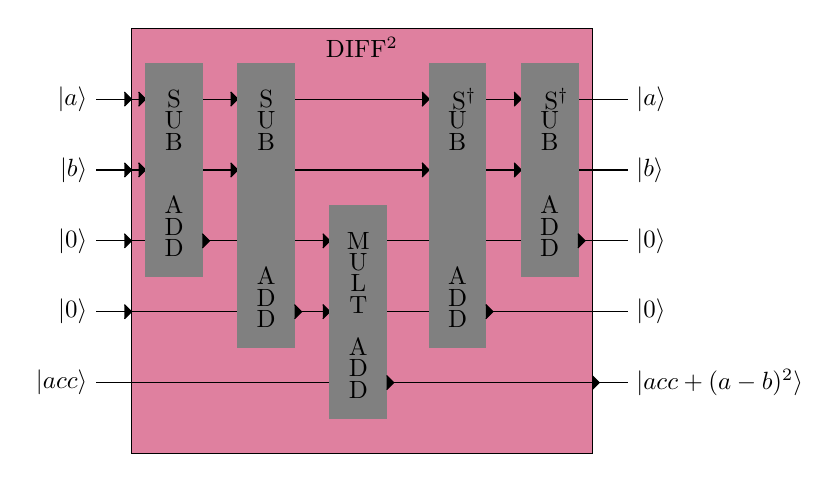
\begin{tikzpicture}[scale=.9, transform shape]
    \filldraw[fill=purple!50] (-1,5) rectangle (5.5,-1) ;
    \node[anchor=north] at (2.25,5) {DIFF$ ^2$};
    \node[rectangle,anchor=east] at (-1.5,4) {$\ket{a}$};
    \node[rectangle,anchor=east] at (-1.5,3) {$\ket{b}$};
    \node[rectangle,anchor=east] at (-1.5,2) {$\ket{0}$};
    \node[rectangle,anchor=east] at (-1.5,1) {$\ket{0}$};
    \node[rectangle,anchor=east] at (-1.5,0) {$\ket{acc}$};

    \node[rectangle,anchor=west] at (6,4) {$\ket{a}$};
    \node[rectangle,anchor=west] at (6,3) {$\ket{b}$};
    \node[rectangle,anchor=west] at (6,2) {$\ket{0}$};
    \node[rectangle,anchor=west] at (6,1) {$\ket{0}$};
    \node[rectangle,anchor=west] at (6,0) {$\ket{acc+(a-b)^2}$};
    \foreach \y in {0,...,4}
        \draw (-1.5,\y) -- (6,\y) ;
    \foreach \y in {1,...,4}
        \filldraw[black] (-1.1,\y-.1) -- (-1,\y) -- (-1.1,\y+.1);
    \filldraw[black] (5.5,-.1) -- (5.6,0) -- (5.5,.1);
    \foreach \x in {0,...,1}{
        \filldraw[black] (\x*1.3-.9,2.9) -- (\x*1.3-.8,3) -- (\x*1.3-.9,3.1);
        \filldraw[black] (\x*1.3-.9,3.9) -- (\x*1.3-.8,4) -- (\x*1.3-.9,4.1);
        \filldraw[gray] (-0.8+\x*1.3,4.5) rectangle (0+\x*1.3,1-\x+.5);
        \filldraw[black] (0+\x*1.3,1-\x+.9) -- (0+\x*1.3+0.1,1-\x+1) -- (0+\x*1.3,1-\x+1.1);
        \node[] at (-0.4+\x*1.3+0,2+2.0) {S}; 
        \node[] at (-0.4+\x*1.3+0,2+1.7) {U}; 
        \node[] at (-0.4+\x*1.3+0,2+1.4) {B}; 
        \node[] at (-0.4+\x*1.3+0,2-\x+.5) {A}; 
        \node[] at (-0.4+\x*1.3+0,2-\x+.2) {D}; 
        \node[] at (-0.4+\x*1.3+0,2-\x-.1) {D}; 
    }

    \filldraw[black] (2*1.3-.9,.9) -- (2*1.3-.8,1) -- (0+2*1.3-.9,1.1);
    \filldraw[black] (2*1.3-.9,1.9) -- (2*1.3-.8,2) -- (0+2*1.3-.9,2.1);
    \filldraw[gray] (-0.8+2*1.3+0,2-2+2.5) rectangle (0+2*1.3,1-2+.5);
    \filldraw[black] (0+2*1.3,1-2+.9) -- (0+2*1.3+0.1,1-2+1) -- (0+2*1.3,1-2+1.1);
    \node[] at (-0.4+2*1.3+0,2.0) {M}; 
    \node[] at (-0.4+2*1.3+0,1.7) {U}; 
    \node[] at (-0.4+2*1.3+0,1.4) {L}; 
    \node[] at (-0.4+2*1.3+0,1.1) {T}; 
    \node[] at (-0.4+2*1.3+0,+.5) {A}; 
    \node[] at (-0.4+2*1.3+0,+.2) {D}; 
    \node[] at (-0.4+2*1.3+0,-.1) {D}; 
    \foreach \x in {0,...,1}{
        \filldraw[black] (4+\x*1.3-.9,2.9+1) -- (4+\x*1.3-.8,3+1) -- (4+\x*1.3-.9,3.1+1);
        \filldraw[black] (4+\x*1.3-.9,1.9+1) -- (4+\x*1.3-.8,2+1) -- (4+\x*1.3-.9,2.1+1);
        \filldraw[gray] (4+-0.8+\x*1.3+0,4.5) rectangle (4+0+\x*1.3,+\x+.5);
        \filldraw[black] (4+0+\x*1.3,+\x+.9) -- (4+0+\x*1.3+0.1,+\x+1) -- (4+0+\x*1.3,+\x+1.1);
        \node[anchor=west] at (-0.4+\x*1.3+4-.2,4.0) {S$ ^\dagger$}; 
        \node[] at (-0.4+\x*1.3+4,2+1.7) {U}; 
        \node[] at (-0.4+\x*1.3+4,2+1.4) {B}; 
        \node[] at (-0.4+\x*1.3+4,1+\x+.5) {A}; 
        \node[] at (-0.4+\x*1.3+4,1+\x+.2) {D}; 
        \node[] at (-0.4+\x*1.3+4,1+\x-.1) {D}; 
    }
\end{tikzpicture}
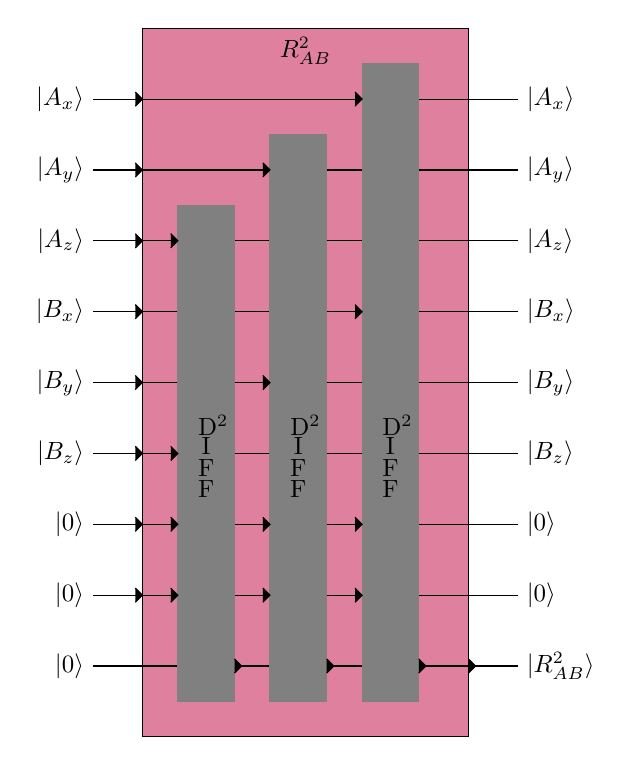
\begin{tikzpicture}[scale=.9, transform shape]
    \filldraw[fill=purple!50] (-1.3,9) rectangle (3.3,-1) ;
    \node[anchor=north] at (1,9) {$R_{AB}^2$};
    
    \node[rectangle,anchor=east] at (-2,8) {$\ket{A_x}$};
    \node[rectangle,anchor=east] at (-2,7) {$\ket{A_y}$};
    \node[rectangle,anchor=east] at (-2,6) {$\ket{A_z}$};
    \node[rectangle,anchor=east] at (-2,5) {$\ket{B_x}$};
    \node[rectangle,anchor=east] at (-2,4) {$\ket{B_y}$};
    \node[rectangle,anchor=east] at (-2,3) {$\ket{B_z}$};
    \node[rectangle,anchor=east] at (-2,2) {$\ket{0}$};
    \node[rectangle,anchor=east] at (-2,1) {$\ket{0}$};
    \node[rectangle,anchor=east] at (-2,0) {$\ket{0}$};

    \node[rectangle,anchor=west] at (4,8) {$\ket{A_x}$};
    \node[rectangle,anchor=west] at (4,7) {$\ket{A_y}$};
    \node[rectangle,anchor=west] at (4,6) {$\ket{A_z}$};
    \node[rectangle,anchor=west] at (4,5) {$\ket{B_x}$};
    \node[rectangle,anchor=west] at (4,4) {$\ket{B_y}$};
    \node[rectangle,anchor=west] at (4,3) {$\ket{B_z}$};
    \node[rectangle,anchor=west] at (4,2) {$\ket{0}$};
    \node[rectangle,anchor=west] at (4,1) {$\ket{0}$};
    \node[rectangle,anchor=west] at (4,0) {$\ket{R_{AB}^2}$};
    \foreach \y in {0,...,8}
        \draw (-2,\y) -- (4,\y) ;
    \foreach \y in {1,...,8}
        \filldraw[black] (-1.4,\y-.1) -- (-1.3,\y) -- (-1.4,\y+.1);
    \filldraw[black] (3.3,-.1) -- (3.4,0) -- (3.3,+.1);
    \foreach \x in {0,...,2}{
        \filldraw[gray] (-0.8+\x*1.3,6.5+\x) rectangle (0+\x*1.3,-.5);
        \filldraw[black] (\x*1.3,-.1) -- (\x*1.3+0.1,0) -- (\x*1.3,.1);
        \foreach \y in {1,2}{
            \filldraw[black] (\x*1.3-.9,\y-.1) -- (\x*1.3-0.8,\y) -- (\x*1.3-.9,.1+\y);
        }
        \foreach \y in {3+\x,6+\x}{
            \filldraw[black] (\x*1.3-.9,\y-.1) -- (\x*1.3-0.8,\y) -- (\x*1.3-.9,.1+\y);
        }
        \node[] at (\x*1.3-0.3,.5+2.9) {D$ ^2$}; 
        \node[] at (\x*1.3-0.4,.5+2.6) {I}; 
        \node[] at (\x*1.3-0.4,.5+2.3) {F}; 
        \node[] at (\x*1.3-0.4,.5+2) {F}; 
    }
\end{tikzpicture}
\caption{Circuits for calculating $a,b,acc\to a,b,acc+(a-b)^2$ and $A,B,0\to A,B, R_{AB}^2$}
\end{figure}
So using this circuit along with a constant addition of $\eta_{AB,ll'}$ and the use of an inverse square root circuit\cite{häner2018} we get a fixed point approximation of $\gamma_{AB,ll'}$. We can use this with our QFT fused multiply add operation to get the inner sum of the $E^\gamma$ term. There could potentially be a lot of pairs, however we can skip almost half with the following rewrite:
\begin{gather}
    \begin{split}
    E^\gamma&=\frac{1}{2}\sum_{A,B}\sum_{l\in A}\sum_{l'\in B} q_lq_{l'}\gamma_{AB,ll'}\\
        &=\sum_{A}\sum_{l\in A}\left[\sum_{l'\in A} q_lq_{l'}\gamma_{AA,ll'}+\sum_{B>A}\sum_{l'\in B} q_lq_{l'}\gamma_{AB,ll'}\right]
    \end{split}
\end{gather}


\subsection{Complexity}
The second algorithm has, in terms of big O notation, the same complexity as the state preparation introduced in the QA-Arithmetic paper, as it is simply 4 applications of this circuit. The state preparation can be achieved using $O(\log n)$ extra qubits and $O(n\log n)$ Toffoli gates where $n$ is the number of bits used to represent $\varGamma_\mu, q_{A_n,\mu}$. Thus if we have a $m$ bit canonical fullerene ID we end up using on the order of $m+2n+4O(\log n)=O(n+m)$ qubits and $4O(n \log n)=O(n \log n)$ Toffoli gates. 

The first circuit on the other hand uses 4 mulitplication circuits, 2 squaring circuits which could just as well be multiplication circuits and an addition circuit. A QFT addition (multiplication) circuit uses $O(n^{2(3)})$ gates and no additional qubits. Thus if we have encoded $\varGamma_{\mu},q_{A_n,\mu}, \mu \in \{0,..,l\}, A_n \in \{0,..,o\}$ each using $n$ bits we will need to perform $6lo$ multiplications and $lo$ additions, resulting in $6lo\cdot O(n^3)+lo\cdot O(n^2)=O(lon^3)$ gates, on $m+n+nl+lon = O(m+lon)$ qubits.
Additionally we then have to run the state preparation circuit which adds $O(\log n)$ qubits and $O(n\log n)$ gates, however that is not enough to change the asymptotic runtime further. 

\subsection{Cleaning up $\omega$}
We would like to get rid of the $\ket{\omega}$ term in both algorithms to avoid having to post select.
We can achieve this with amplitude amplification. 
To do amplitude amplification we first need to define what a 'good' state is, in our case we know all good states have $\ket{0}_C\ket{1}_W$. 
Second we need an oracle in terms of a unitary which flips the sign of the good state, i.e. reflecting the state around the bad state, this would be $I-2\ket{0}_C\bra{0}_C\ket{1}_W\bra{1}_W$, which can be easily implemented with controlled rotations. 
We also need a circuit which would reflect around the initial state by flipping the sign of it, given that we have a circuit $U$ for preparing the initial state that would be $I-2U\ket{0}\bra{0}U^\dagger$.
In our case the angle between the bad and initial states are $\theta_{DA} = arcsin(\frac{1}{2}\frac{E^\Gamma}{2^n}),\theta_{AA} = arcsin(\frac{1}{2^4}\frac{E^\Gamma}{2^{n4}})$ for the two algorithms. We have to do $\lfloor\frac{\pi}{4\theta}\rfloor$ repetitions to maximize the probability of measuring a good state.%Todo: fix every calculation and number in this. the propably all wrong 
\subsection{Concentrating the probabilities on the best candidates}
We now have a superposition where the probability of sampling a fullerene is proportional to the energy of that fullerene.
But is that ideal? The energies might be quite close to each other in absolute terms.
Therefore we would like to exaggerate the difference between them and then sample according to that difference.
If we knew what the highest energy was we could just subtract that from every energy calculation thus getting probabilities proportional to how much lower an energy we are working with.
Another option is if we expect the energies to be within $100(1-x)\%$ we could subtract $ex$ from every energy calculation where $e$ is the energy from a random fullerene in the isomer-space.
This is of cause not as good but quite achievable. In both algorithms we can encode $ex$ in a register and then use a digital subtraction or do a QAA state preparation addition but with all the $R_y$ gates inverted, resulting in a counter-clockwise rotation, in effect subtracting $ex$.
%Note: the following is dumb, we don't want to invert the probabilities! 
%If we expect the results from these shifted energy calculations to be in the interval $]0,1[$ we can exaggerate them further by taking the reciprocal. 
\subsection{Discussion}
From the asymptotic resource use the second algorithm is clearly superior, even if some of the multiplications and additions can be run in parallel in the first one. We do have a factor 8 lower chance of getting a useful state out, but this again does not change the asymptotics, as we can just repeat it. 
QA-Amplification might be possible since we have a very clear "good" state in both algorithms. This would reduce the need for postselection and repetitions. Preparing the initial encoding of the isomer space seems less straight forwards in the second approach than in the first unfortunately. 

\chapter{Related Work}

\section{xtb version 6.4.0}
The xtb project has basic GPU support through the Nvidia Fortran compiler 'nvfortran', but this compiler fails on newer versions of the project. To get a version that has been officially tested with nvfortran, we have to go all the way back to version 6.4.0 from Feburary 2021.
We have successfully made a reproducable build for this version and managed to run it, but the output seems much different from newer versions. There has been released 7 versions since, so doing any benchmarking comparisons with this older version likely would not be fair or representative.

\section{dxtb}
The dxtb project is a re-implementation of the xTB methods written in Python. This implementation has much better comments that actually explain the functions, but we discovered the project late into the process, and as such it has not been hugely beneficial for us.
The project is no substitute for a GPU implementation, but it could have helped us with our own Python re-implementation.

\section{Methodology}

\subsection{Testing}

The xTB algorithm computes a lot of different energies, corrections, and other additions to the energy terms. There is a lot of overlap between the different variants of xTB, so even focusing on just one of them still requires a great amount of code.
Dealing with large computations with so many small parts makes proper validation especially important, as it becomes increasingly easy to make mistakes.
In the case of the xTB algorithm, the original Fortran implementation becomes an important point of reference for comparison. Throughout the coding process it became apparent that the xTB implementation by the Grimme research group does not match the equations described in the original xTB paper by the same authors.

% TODO: Give examples of code that does not follow the paper!

With this realization the obvious approach forward was to lean towards the existing implementation rather than the paper. This choice would allow us to continue doing validation against the existing code as a reference.

One of the hurdles from testing against an existing program becomes the lack of transparency regarding the logic that takes place between the initial input and the final output presented to the user. Thankfully, the source code is publicly available allowing for easy manipulation of the original flow of execution, thus avoiding the hassle of testing against a black box or the need to resort to methods of reverse engineering.

On behalf of these considerations it was decided to write patches that allow to intercept the arguments and results of arbitrary functions just by running the program as normal. This meant that smaller parts could be implemented without the need to implement all the code needed to compute its arguments.

An important part of any software is reproducability, and applying certain patches in certain scenarios is something that should preferably be automated, reproducable, and optimally also portable. This is especially important for this approach to validation as it requires a way to reproduce a specific version of xTB linked to the same versions of dependencies. Essentially an exact copy of the original shell environment to ensure that patches work, results are the same, and no new bugs appear in the program itself or its dependencies. All of this should be achievable without having to add, remove, downgrade or upgrade system packages on your system.

The well-known contenders for this is any of the numerous containerization solutions on Linux, such as Docker, Podman, LXC etc. There are some problems with these options though, one being that it can be difficult to truly reproduce package versions without saving the resulting container image, another being that it does not solve the problem of having multiple versions of the same package installed. Some other notable limitations are that it limits the process to run within the container and passing in a GPU or other hardware can be nefariously difficult. A container also does not have access to the X or Wayland session needed to run GUI applications, though that is not currently relevant in this case.

Another approach which has been growing in popularity in recent years are tools that take unique approaches to package management in order to make not only packages reproducable, but also shell environments, system configurations and other forms of "outputs". Two such popular package managers are Nix from the Nix team and Guix from the GNU foundation. Nix is arguably the more popular option and it is also the solution that has been chosen for this project.

Nix is an umbrella term that can refer to either the Nix functional programming language, the package manager, or the Nix based Linux distribution NixOS. The language and package manager go hand in hand and can be used on any Linux distribution. As such, NixOS is not required for the needs of this project and will not be mentioned going forward.

Nix does not follow the Unix Filesystem Hierarchy Standard (FHS), which brings with it some challenges, but this fundamental difference from other package managers is a major part of what makes Nix so powerful.
Rather than installing packages into the usual system paths like `/bin`, `/lib` etc. Nix installs everything into a read-only path called the Nix store under `/nix/store`.
Everything in the Nix store is a result of a core concept in Nix called a derivation, which is essentially a build task to produce some output of files into the Nix store.
All outputs into the store is marked with a custom hash in the filename called a NAR hash. These fundamental ideas fix some common problems such as circular dependencies and allow having multiple versions of the same package installed as they will simply coincide in the Nix store with different NAR hashes.

The typical binary on Linux is dynamically linked against the FHS compliant paths and it is not uncommon to have them hardcoded either. To make use of the packages in the Nix store, it is required to either recompile the program against the store paths, or in the case of proprietary software, patching the ELF header is needed to change the path to the interpreter and to dynamically linked libraries. Thankfully the Nix package repository 'NixPkgs' is the largest and freshest out there\footnote{\url{https://repology.org/repositories/graphs}}, so as a typical user doing this is rarely needed.
Nixpkgs is a version-controlled repository on GitHub, so using older versions of packages even alongside newer ones, is fairly trivial as it simply requires fetching multiple revision of the repository.

This along with the previously mentioned features have allowed a greatly simplified process of not only running the newest version 6.7.1 of the xTB program, but also running the much older nvfortran compatible version 6.4.0 alongside it.
NixPkgs is also a collection of library functions, and the helper functions for making derivations called `mkDerivation` make it easy to define all the stages of packaging a program including unpacking, patching, building, checking, and installing the files.
With this, the whole pipeline of patching, compiling, running, and passing the data over to the Python validation tests can be achieved with a single shell command.

\begin{minted}{bash}
nix run .#cmp-impls
\end{minted}


This command takes the form '\verb|nix run <path to flake>#<output>|'. Path to flake refers to a file-tree whose root directory contains a file called 'flake.nix'. Nix flakes is an experimental but widely adopted feature, which provides a standard way to write Nix expressions and a way to manager their dependencies through a version-pinned lock file. The 'flake.nix' file follows a uniform naming schema for declaring inputs and outputs, where inputs are the dependencies, and outputs are Nix expressions to be exposed.
The new Nix command-line interface needed to interact with flakes is naturally also an experimental feature that has to be enabled explicitly. The run command instructs Nix to build and run the derivation 'cmp-impls', which is defined as an app in the flake outputs.

\newpage

\begin{minted}{nix}
{
  inputs = {
    nixpkgs.url = "github:nixos/nixpkgs/nixos-unstable";
  };

  outputs = { self, nixpkgs, ... }: {
    apps."x86_64-linux" = let
      pkgs = nixpkgs.legacyPackages."x86_64-linux";
      ...
    in {
      "cmp-impls" = let
        python = (pkgs.python3.withPackages (python-pkgs: with python-pkgs; [
          numpy scipy cvxopt
        ]));
      in {
        type = "app";
        program = toString (pkgs.writeShellScript "cmp-impls" ''
          PYTHONPATH=${pkgs.lib.cleanSource ./xtb-python} exec ${python}/bin/python \
            ${./xtb-python/cmp_impls.py} ${xtb_test_data}
        '');
      };
    };
    ...
  };
}
\end{minted}

Python is declared with the required packages and is then used in the app to call the \verb|cmp_impls.py| script. The script is called with the test data acquired from running the Fortran xTB program. This data comes from another derivation which executes patched versions of xTB and DFT-D4 on a C200 fullerene to get the relevant function arguments and results as binary files.

\begin{minted}{nix}
xtb_test_data = builtins.derivation {
  name = "xtb-test-data";
  system = "x86_64-linux";
  builder = "${pkgs.bash}/bin/bash";
  src = ./xtb-python/data/C200.xyz;
  args = ["-c" ''
    PATH=$PATH:${pkgs.coreutils}/bin
    mkdir -p ./calls/{build_SDQH0,coordination_number,\
      dim_basis,dtrf2,electro,form_product,get_multiints,\
      h0scal,horizontal_shift,multipole_3d,newBasisset, olapp}
    ${xtb}/bin/xtb $src
    ${dftd4}/bin/dftd4 $src
    mv calls $out
  ''];
};
\end{minted}

The directories for the binary files are created in advance as checking whether they exist when writing the binary files has a large overhead.
This derivation in turn uses derivations for xTB and DFT-D4. Luckily DFT-D4 is already in NixPkgs, but it still needs to be patched in order to extract the required data for validation. Thankfully the \verb|mkDerivation| function used in NixPkgs makes overriding and patching a package very straightforward. 

\begin{minted}{nix}
dftd4 = (pkgs.dftd4.overrideAttrs (finalAttrs: previousAttrs: {
  src = pkgs.fetchFromGitHub {
    owner = "dftd4";
    repo = "dftd4";
    rev = "502d7c59bf88beec7c90a71c4ecf80029794bd5e";
    hash = "sha256-FEABtBAZK0xQ1P/Pbj5gUuvKf8/ZLITXaXYB+btAY/8=";
  };
  buildInputs = [ multicharge ] ++ previousAttrs.buildInputs;
  doCheck = false;
  patches = previousAttrs.patches ++ [
    ./nix/patches/dftd4/use_gfn2.patch
    ./nix/patches/dftd4/log_args_and_outputs.patch
  ];
}));
\end{minted}

The version is bumped by overriding the source, and the multicharge project is added from NixPkgs and also bumped as a requirement of this newer version. Some of the tests were timing out, so they have been disabled by setting \verb|doCheck| to false. Lastly the patches are applied by providing the relevant patch files.


xTB and two of its dependencies, namely CPCM-X and numsa are not in NixPkgs and had to be packaged from scratch.

All the patches follow the structure below where the original function is prefixed with a 'g', such that the new wrapper function will be called instead. The wrapper function writes the function arguments to a binary file before calling the actual function and then finally writes the result to the same file.
Writing a file for each call to a function is a bit excessive and will produce a very large amount of files, so a threshold has been used to create an upperbound on the number of files that can be created for each function.

\begin{minted}{diff}
+   logical :: hit_threshold
+   integer :: u
+   character(len=200) :: path
+
+   hit_threshold = testfile_path('electro', path)
+   if (.not.hit_threshold) then
+     open(newunit=u, file=trim(path), form='unformatted', access='stream')
+     write(u) nbf
+     write(u) size(H0), H0
+     write(u) size(P, 1), size(P, 2), P
...
+     if (allocated(ies%thirdOrder%atomicGam)) then
+       write(u) size(ies%thirdorder%atomicgam), ies%thirdorder%atomicgam
+     else
+       write(u) 0
+     end if
...
+     write(u) size(ies%jmat, 1), size(ies%jmat, 2), ies%jmat
+     write(u) size(ies%shift), ies%shift
+   end if
+
+   call gelectro(n,at,nbf,nshell,ies,H0,P,dq,dqsh,es,scc)
+
+   if (.not.hit_threshold) then
+     write(u) es
+     write(u) scc
+     close(u)
+   end if
\end{minted}

When all the data has been written, then the binary files are passed onto \verb|cmp-impls.py|, which is the test suite for comparing the Python reimplementation to the original Fortran code. 

\begin{minted}{python}
def test_electro():
    fn_name = "electro"
    for i, file_path in enumerate(glob.glob(f'{directory}/{fn_name}/*.bin')):
        with open(file_path, 'rb') as f:
            def read_ints(n=1):
                return np.fromfile(f, dtype=np.int32, count=n)

            nbf = read_ints(1)[0]
            H01 = read_ints(1)[0]
            H0 = np.fromfile(f, dtype=np.float64, count=H01)
            m, n = read_ints(2)
            P = np.fromfile(f, dtype=np.float64, count=m * n).reshape((n, m))
            ...
            atomicGam1 = read_ints(1)[0]
            atomicGam = None  if atomicGam1 == 0
                              else np.fromfile(f, dtype=np.float64, count=atomicGam1)
            ...
            es_res, scc_res = read_reals(2)
            es, scc = electro(nbf, H0, P, dq, dqsh, atomicGam, shellGam, jmat, shift)

            is_equal(es, es_res, "es", fn_name)
            is_equal(scc, scc_res, "scc", fn_name)

    print(f"matches! [{fn_name}]")
\end{minted}

\chapter{Results}

\section{Our Contributions}

In this section we will present and reiterate the contributions we have made as a result of this project.

We have contributed with a simplified Python version of the original GFN2-xTB Fortran implementation. The implementation and validation of the dispersion, anisotropic and Fermi terms is not complete, and we have not implemented the self-consistent charges that is used to iteratively rerun the computations to improve the accuracy of the result. Given the size of the reference implementation we are quite satisfied with this progress. The Python implementation should hopefully make the GFN2-xTB algorithm more approachable for our successors and give a good foundation for making a lock-step parallel GPU implementation.

We have contributed a testing framework for comparing results against the original Fortran implementation. We utilize Nix to ensure tests that are reproducible, regardless of Linux distribution and system configuration. In connection to this, we have also contributed a reproducible and easy way to build, run, and patch xtb. This also includes its dependencies, and even the older GPU compatible version 6.4.0 of xtb known from GitHub issues to be difficult to get up and running.

This thesis contributes an in-depth walk-through of the GFN2-xTB algorithm with code snippets that directly link to the equations in a way that should be more easily digestible for a computer scientist. As an extension of this, we have presented insights and ideas on how to approach a massively lock-step implementation by optimizing code snippets for our problem domain, and transforming them such that they adhere to the requirements of a lock-step kernel.

We have also presented a case study with the NVIDIA A100 data centre GPU to show how GPU architectures are structured and how to use the technical specifications to estimate hardware requirements.

Additionally we have designed quantum circuits for computing the isotropic energy terms in GFN2-xTB, with some theoretic advantages in sampling. These could be used as a starting point for a fully quantum computational approach. 

\section{Validation}

All of our tests pass indicating that our results match the reference implementation. We had to introduce a threshold for some of the comparisons as they came extremely close. \autoref{fig:validation_electro_precision} shows the maximum squared deviations of all tests for the electrostatic term. This term returns the isotropic electrostatic energy and the self-consistent charges, so there are two plots to show both.

\begin{figure}[H]
\centering
\begin{subfigure}{.5\textwidth}
  \centering
  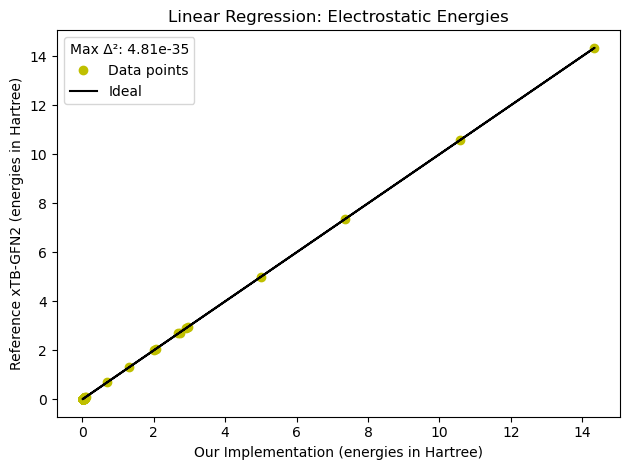
\includegraphics[width=.9\linewidth]{images/results/es_check}
  \label{fig:es_check}
\end{subfigure}%
\begin{subfigure}{.5\textwidth}
  \centering
  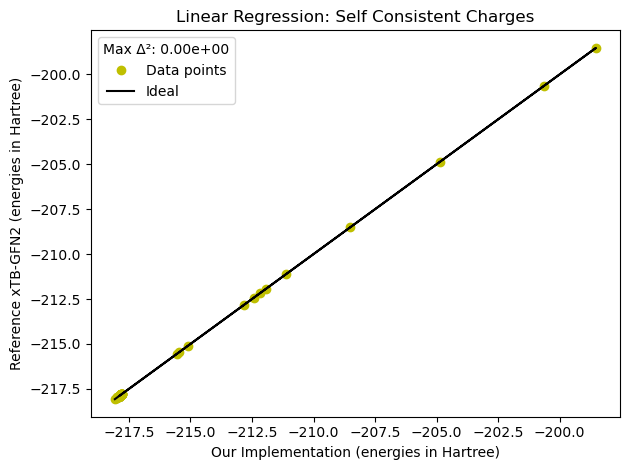
\includegraphics[width=.9\linewidth]{images/results/scc_check}
  \label{fig:scc_check}
\end{subfigure}
\caption{Linear regressions showing how much the Python implementation for the electrostatic term deviates from the Fortran results.}
\label{fig:validation_electro_precision}
\end{figure}

\section{Benchmarks}

\chapter{Reflections}\label{sec:reflection}
In this section we will reflect on our choices and approaches to highlight what we think worked well. We will also share possible changes worth considering for anyone pursuing to continue this project.%We will also share changes in the landscape that have occured since the start of this project.

We have primarily made use of the Python programming language for the prototype implementation of GFN2-xTB. This has worked well due to Python's simple syntax, runtime checks, and abstractions of low-level details such as memory management. These traits have let us focus on correctness rather than specifics about the code and language.

The package manager and functional language Nix has given us similar advantages by providing us with reproducable development environments, a flexible solution for software packaging, and a way to combine this to make a reproducable testing pipeline. %Because of this, we have been able to focus on troubleshooting the actual implementation rather than system specific problems.

Nix is known to have a rather steep learning curve, which deters many, but given our experiences, we can wholeheartedly recommend this workflow. The testing setup with Nix has been especially valuable, continuing to pay dividends by ensuring correctness as we transition from a prototype to a high performance implementation.

The xTB family of algorithms presented by Grimme et al. is still being actively developed. In fact g-xTB came out a little over half way though this project and is rather impressive regarding accuracy and breadth of application. We urge anyone continuing this project to consider if the resulting changes impact fullerenes enough to warrant switching to the new method. We were unable to make this assessment as the reference implementation has still not landed in the tblite repository, and the associated paper is still only a preprint available on chemRxiv\cite{g-xtb}. 
The eventual advent of g-xTB may justify adapting our work to the new method. 

Completing the Python prototype is highly relevant as it is a crucial step towards the main prize of a fully lockstep-parallel implementation of the algorithm. 
An interesting stand-alone part of the method is implementing the D4' dispersion model. 

Slightly outside of the project scope, we would like to extend the prototype from just computing the energy terms mentioned to include also polarization and excitation energies. Implementing at least one of the solvation models available in the xtb program would also be a welcome addition. The current prototype handles everything as one 'cell', perfect for simulating individual molecules, however extending it to handle repeating cells, such as in crystals, should be a rather small change. 

Regarding quantum algorithms we want to investigate using quantum singular value decomposition transforms for some of the terms that are more heavy on tensors. This would be a good thesis topic for anyone interested in quantum algorithm design. It would also be interesting to investigate if any of the approximations in GFN2-xTB are unnecessary in the domain of quantum computing.

%\chapter{Future Work}

%\section{Extended Hückel Theory Matrix for GFN2-xTB}
\begin{equation}
\begin{split}
    \mn{H^{EHT}} &= \frac{1}{2}K^{ll'}_{AB}\mn{S}(H_{\mu\mu}+H_{\nu\nu})\\&\cdot X(EN_A,EN_B)\\&\cdot \Pi(R_{AB},l,l')\\&\cdot Y(\zeta^A_l,\zeta^B_{l'}), \forall \mu \in l(A), \nu \in l'(B)
\end{split}
\end{equation}
where $\mu$ and $\nu$ are AO indecies, $l$ and $l'$ index shells. Both AO's are associated with an atom labled A and B. 
$K^{ll'}_{AB}$ is a element and shell specific fitted constant however, in GFN2 it only depends on the shells. 
$S_{\mu\nu}=\braket{\phi_\mu|\phi_\nu}$ is just the overlap of the orbitals. In GFN2 $H_{\kappa\kappa}=h^l_A-\delta h^l_{CN'_A}CN'_A$ where $CN'_A$ is the modified GFN2-type Coordinate Number for the element of atom A.

\begin{align}
\begin{split}
  CN^{'}_A = &\sum^{N_\text{atoms}}_{B \neq A} (1 + e^{-10(4(R_{A,\text{cov}} + R_{B,\text{cov}})/3R_{AB}-1)})^{-1} \\
             &\times (1 + e^{-20(4(R_{A,\text{cov}} + R_{B,\text{cov}} + 2)/3R_{AB}-1)})^{-1}
\end{split}
\end{align}

$h^l_A$ and $\delta h^l_{CN'_A}$ are both fitted constants. $EN_A$ is the electronegativity of the element of atom A, given in the original \texttt{xtb} code. 

\begin{align}
    X(EN_A,EN_B) &= 1 + k_{EN}\Delta EN_{AB}^2\\
    k_{EN} &= 0.02 \text{ in GFN2}\\
    \Delta EN_{AB}^2 &= (EN_A-EN_B)^2  
\end{align}
%The electronegativity for C and H are 2.55 and 2.20 according to wikipedia.
%Thus here is a table for the combinations we will be working with:\\ 
%\begin{tabular}{c|c|l}
%    A&B&$X(EN_A,EN_B)$\\
%    \hline
%    C&C&$1$\\
%    C&H&$1+0.02\cdot (0.35^2)$\\
%    H&C&$1+0.02\cdot (0.35^2)$\\
%    H&H&$1$\\
%\end{tabular}
\begin{equation}
\begin{split}
    \Pi(R_{AB},l,l') &= \left(1 + k^{\text{poly}}_{A,l}\left(\frac{R_{AB}}{R_{\text{cov},AB}}\right)^\frac{1}{2}\right)\left(1 + k^{\text{poly}}_{B,l'}\left(\frac{R_{AB}}{R_{\text{cov},AB}}\right)^\frac{1}{2}\right)\\
\end{split}
\end{equation}
$R_{\text{cov},AB}$ are the summed covalent radii (\(R_{\text{cov},A} + R_{\text{cov},B}\)), e.g. $R_{\text{cov},H}=0.32$, $R_{\text{cov},C}=0.75$ are given in the original \texttt{xtb} code. $k^{\text{poly}}_{A,l}$ and $k^{\text{poly}}_{B,l'}$ are element and shell specific constants. 
\begin{equation}
\begin{split}
    Y(\zeta^A_l,\zeta^B_{l'}) &= \left(\frac{2\sqrt{\zeta^A_l\zeta^B_{l'}}}{\zeta^A_l+\zeta^B_{l'}}\right)^\frac{1}{2}\\
\end{split}
\end{equation}
Here, $\zeta^A_l$ are the STO exponents of the GFN2-xTB AO basis.\\
Slater Type Orbitals are defined as such: 
\begin{equation}
\chi_{\zeta,n,l,m}(r, \theta, \varphi) = NY_{l,m}(\theta, \varphi)r^{n-1}e^{-\zeta r}
\end{equation}
N is a normalisation constant, Y are spherical harmonic funtions, n, l, m are the quantum numbers for the AO. $r,\theta,\varphi$ are polar 3D coordinates. $\zeta$ determines the radial extent of the STO, a large value gives rise to a function that is "tight" around the nucleus and a small value gives a more "diffuse" function. This $\zeta$ is the one mentioned in the Y term of $\E{EHT}$ and is a value fitted when constructing the basis set, thus it is given to us.  


%\section{Fock Matrix for GFN2-xTB}
\begin{equation}
\begin{split}
    \mn{F^{GFN2-xTB}} =  \mn{H^{EHT}} + \mn{F^{IES+IXC}} + &\mn{F^{AES}}+\mn{F^{AXC}}+\mn{F^{D4}}, \\&\forall \mu \in A, \nu \in B
\end{split}
\end{equation}
\subsection{Isotropic Electrostatic and Exchange-correlation contribution}
\begin{equation}
\begin{split}
    \mn{F^{IES+IXC}} = &- \frac{1}{2}\mn{S}\sum_C\sum_{l''}(\gamma_{AC,ll''}+\gamma_{BC,l'l''})q_{C,l''}\\
    &-\frac{1}{2}\mn{S}(q_{A,l}^2\Gamma_{A,l}+q_{B,l'}^2\Gamma_{B,l'})
\end{split}
\end{equation}
$l,l',l''$ being the angular momenta of the orbitals $\mu, \nu$ and each of C's orbitals. 
\begin{equation}
    \Gamma_{A,l} = K^\Gamma_l\Gamma_A
\end{equation}
$K^\Gamma_l$ is a shell specific constant common for all elements and $\Gamma_A$ is an element specific constant. 
\begin{align}
    \gamma_{AB,ll'} &= \frac{1}{\sqrt{R_{AB}^2+\eta^{-2}_{AB,ll'}}}\\
    \eta_{AB,ll'}&=\frac{1}{2}\left[\eta_A(1+k_A^l)+\eta_B(1+k_B^{l'})\right]
\end{align}
$q_l$ is a partial Mulliken charge. $\eta_A$ and $\eta_B$ are element-specific fit parameters, while $k_A^l$ and $k_B^{l'}$ are element-specific scaling factors for the individual shells ($k_A^l=0$ when $l=0$).
\begin{align}
    GAP_A &= \sum_{l \in A} q_{A,l}\\
    q_{A,l} &= \sum_{l'\in B}P_{ll'}S_{ll'} = GOP_l
\end{align}

\subsection{Anisotropic Electrostatic and Exchange-correlation contribution}
\begin{align}
    \begin{split}
    \mn{F^{AES}}+\mn{F^{AXC}} &= \frac{1}{2}\mn{S}\left[V_S(\pmb{R}_B)+ V_S(\pmb{R}_C)\right]\\
    &+ \frac{1}{2}\mn{\pmb{D}^T}\left[\pmb{V}_D(\pmb{R}_B)+\pmb{V}_D(\pmb{R}_C)\right]\\
    &+ \frac{1}{2} \sum_{\alpha,\beta\in\{x,y,z\}} \mn{Q^{\alpha\beta}}\left[V_Q^{\alpha\beta}(\pmb{R}_B)+ V_Q^{\alpha\beta}(\pmb{R}_C)\right]
    \end{split}\\
    \mn{\pmb{D}^T} &=
    \begin{pmatrix}
        \mn{D^x} &
        \mn{D^y} &
        \mn{D^z}\\
    \end{pmatrix}\\
\end{align}
\begin{align}
    \begin{split}
        V_S(\pmb{R}_C)& = \sum_A \Biggl\{
        \pmb{R}_C^T\biggl[
            f_5(R_{AC})\pmb{\mu}_AR^2_{AC} - 
            \pmb{R}_{AC}3f_5(R_{AC})(\pmb{\mu}_A^T\pmb{R}^2_{AC}) \\&- 
            f_3(R_{AC})q_A\pmb{R}_AC
        \biggr] 
    - f_5(R_{AC})\pmb{R}^T_{AC}\pmb{\Theta}_A\pmb{R}_{AC}
          - f_3(R_{AC})\pmb{\mu}^T_{A}\pmb{R}_{AC}\\
          &+q_Af_5(R_{AC})\frac{1}{2}\pmb{R}_C^2\pmb{R}_{AC}^2 
          - \frac{3}{2}q_Af_5(R_{AC})\sum_{\alpha\beta}\alpha_{AB}\beta_{AB}\alpha_{C}\beta_{C}\Biggr\}\\
      &+2f_{XC}^{\mu_C}\pmb R^T_C\pmb\mu_C - f_{XC}^{\Theta_C}\pmb R^T_C\biggl[3\pmb\Theta_C-\text{Tr}(\pmb\Theta_C)\pmb I\biggr]\pmb R_C
    \end{split}
\end{align}
\begin{align}
    \begin{split}
        V_D(\pmb{R}_C)
            &= \sum_A \Biggl[
                \pmb{R}_{AC}3f_5(R_{AC})(\pmb{\mu}_A^T\pmb{R}_{AC}) -
                f_5(R_{AC})\pmb{\mu}_AR^2_{AC} + 
                f_3(R_{AC})q_A\pmb{R}_{AC}\\
            &-q_Af_5(R_{AC})\pmb{R}_CR_{AC}^2 + 
                3q_Af_5(R_{AC})\pmb{R}_{AC}\sum_\alpha\alpha_C\alpha_{AC}\Biggr]\\
      &-2f_{XC}^{\mu_C}\pmb\mu_C - 2f_{XC}^{\Theta_C}\biggl[3\pmb\Theta_C-\text{Tr}(\pmb\Theta_C)\pmb I\biggr]\pmb R_C
    \end{split}
\end{align}
\begin{align}
    \begin{split}
        V_Q^{\alpha\beta}(\pmb{R}_C)
            &= -\sum_A q_Af_5(R_{AC})\left[          
                \frac{3}{2}\alpha_{AC}\beta_{AC}- \frac{1}{2}R_{AB}^2 % TODO: is AB correct here!?
                \right]\\
        &-f_{XC}^{\Theta_C}\left[3\pmb\Theta_C^{\alpha\beta}-\delta_{\alpha\beta}\sum_\alpha\pmb\Theta_C^{\alpha\alpha}\right]
    \end{split}
\end{align}

$\pmb{\mu}_A$ is the cumulative atomic dipole moment of atom A and $\pmb{\Theta}_A$ is the corresponding traceless quadrupole moment. Traceless simply means that the sum of the diagonal elements is 0. The curly braces and brackets are used in the same way as normal parenthesis for showing order of operations. $q_A$ is the atomic charge of atom A. 
\begin{align}
    \Theta_A^{\alpha\beta} &= \frac{3}{2} \theta_A^{\alpha\beta} - \frac{\delta_{\alpha\beta}}{2} \left( \theta_A^{xx} + \theta_A^{yy} + \theta_A^{zz} \right)\\
    \theta_A^{\alpha\beta} &= \sum_{l' \in A} \sum_{l} P_{l} \left( \alpha_A D_{ll'}^{\beta} + \beta_A D_{ll'}^{\alpha} - \alpha_A \beta_A S_{ll'} - Q_{ll'}^{\alpha\beta} \right)\\
    q_A &= Z_A - GAP_A\\
    \mu_A^{\alpha} &= \sum_{l' \in A} \sum_{l} P_{l'l} \left( \alpha_A S_{l'l} - D_{l'l}^{\alpha} \right)\\
D_{ll'}^{\alpha} &= \braket{ \phi_{l} | \alpha_i | \phi_{l'}}\\
Q_{ll'}^{\alpha\beta} &= \braket{ \phi_{l} | \alpha_i\beta_i | \phi_{l'}}
\end{align}
$\alpha$ and $\beta$ are Cartesian components labled $(x,y,z)^T$ with atom A being centered in $\pmb{R}_A = (x_i,y_i,z_i)^T$ where i is a form of pointer/label dereferencing. $\delta_{\alpha\beta}$ is just the delta function, i.e is is 1 if $\alpha$ and $\beta$ are the same label and 0 otherwise, this serves to include the term only for the diagonal. 

\begin{equation}
    \pmb{\Theta}_A = 
    \begin{pmatrix}
        \Theta_A^{xx} & \Theta_A^{xy} & \Theta_A^{xz}\\
        \Theta_A^{yx} & \Theta_A^{yy} & \Theta_A^{yz}\\
        \Theta_A^{zx} & \Theta_A^{zy} & \Theta_A^{zz}\\
    \end{pmatrix}
\end{equation}
\begin{equation}
    \pmb{\mu}_A = 
    \begin{pmatrix}
        \mu_A^{x}&
        \mu_A^{y}&
        \mu_A^{z}\\
    \end{pmatrix}^T
\end{equation}
\begin{align}
    \pmb{R}_{AB} &= \pmb{R}_A-\pmb{R}_B\\
    R_{AB} &= \sqrt{(\pmb{R}^x_{AB})^2+(\pmb{R}^y_{AB})^2+(\pmb{R}^z_{AB})^2}
\end{align}


\begin{align}
    f_n(R_{AB}) &= \frac{f_{damp}(a_n,R_{AB})}{R_{AB}^n}=\frac{1}{R_{AB}^n}\frac{1}{1+6\left(\frac{R_0^{AB}}{R_{AB}}\right)^{a_n}}\\
    R_0^{AB} &= 0.5 ({R^A_0}'+ {R^B_0}')\\
    {R^A_0}' &= \begin{cases}R^A_0 + \frac{R_{max}-R^A_0}{1+exp[-4(CN_A'-N_{val}-\Delta_{val})]} & \text{if }N_{val}\text{ is given}\\5.0 \text{ bohrs} & \text{otherwise}\end{cases}\\
        R_{max} &= 5.0 \text{ bohrs}\\
    \Delta_{val} &= 1.2
\end{align}
$R_0^A$ is a fitted value for 12 elements and 5.0 for the rest. $a_n$ are adjusted global parameters. 
Where $f^{\mu_A}_{XC}$ and $f^{\Theta_A}_{XC}$ are fitted values. 
\subsection{Dispersion contribution}
\begin{align}
    \mn{F^{D4}} &= -\frac{1}{2}\mn{S}(d_A+d_B), \forall \mu \in A, \nu \in B\\
\begin{split}
    d_A &= \sum_r^{N_{A,ref}} \frac{\partial \xi^r_A(q_A,q_{A,r})}{\partial q_A}\sum_B\sum_s^{N_{B,ref}}\sum_{n=6,8}\\
    &\quad\quad W_A^r(CN^A_{cov},CN^{A,r}_{cov})W_B^s(CN^B_{cov},CN^{B,s}_{cov})\xi^s_B(q_B,q_{B,s})\times\\
    &\quad\quad s_n\frac{C^{AB,ref}_n}{R_{AB}^n}f_n^{damp,BJ}(R_{AB}) 
\end{split}
\end{align}

The dispersion coefficient for two reference atoms \(C_n^{AB,\text{ref}}\) is evaluated at the reference points, i.e., for \(q_A = q_r\), \(q_B = q_s\), \(CN_{\text{cov}}^A = CN_{\text{cov}}^r\), and \(CN_{\text{cov}}^B = CN_{\text{cov}}^s\).

\vspace{10pt}
\noindent
The Gaussian weighting for each reference system is given by:
\begin{equation}
  W_A^r(CN_{cov}^A, CN_{cov}^{A,r}) = \sum_{j=1}^{N_{gauss}} \frac{1}{\mathcal{N}} \exp\left[-6j \cdot (CN_{cov}^A - CN_{cov}^{A,r})^2\right]
\end{equation}

with
\begin{equation}
  \sum_{r}^{N_{A,ref}} W_A^r(CN_{cov}^A, CN_{cov}^{A,r}) = 1
\end{equation}

\vspace{10pt}
\noindent
\(\mathcal{N}\) is a normalization constant.

\noindent
The number of Gaussian function per reference system \(N_{gauss}\) is mostly one, but equal to three for \(CN_{cov}^{A,r} = 0\) and reference systems with similar coordination number.


\vspace{10pt}
\noindent
\(C_6^{AB}\) is the pairwise dipole-dipole dispersion coefficients calculated by numerical integration via the Casimir-Polder relation.
\begin{equation}
  C_6^{AB} = \frac{3}{\pi} \sum_{j} w_j \overline{\alpha}_A (i\omega_j, q_A, CN_{cov}^A)\overline{\alpha}_B (i\omega_j, q_B, CN_{cov}^B)
\end{equation}

\noindent
\(w_j\) are the integration weights, which are derived from a trapeziodal partitioning between the grid points \(j(j \in [1,23])\).

\noindent
The isotropically averaged, dynamic dipole-dipole polarizabilites \(\overline{\alpha}\) at the \(j\)th imaginary frequency \(i\omega_j\) are obtained from the self-consistent D4 model; i.e., they are depending on the covalent coordination number and are also charge dependent.

\begin{equation}
  \overline{\alpha}_A(i\omega_j, q_A, CN_{cov}^A) = \sum_{r}^{N_{A,ref}} \xi_A^r (q_A, q_{A,r}) \overline{\alpha}_{A,r}(i\omega_j, q_{A,r}, CN_{cov}^{A,r}) W_A^r(CN_{cov}^A, CN_{cov}^{A,r})
\end{equation}

\noindent
The charge-dependency is included via the empirical scaling function \(\xi_A^r\).
\begin{equation}
  \xi_A^r(q_A, q_{A,r}) = \exp\left[3\left\{1-\exp\left[4\eta_A\left(1-\frac{Z_A^{eff} + q_{A,r}}{Z_A^{eff} + q_A}\right)\right]\right\}\right]
\end{equation}

\noindent
where \(\eta_A\) is the chemical hardness taken from ref 98.

\noindent
\(Z_A^{eff}\) is the effective nuclear charge of atom A, which has been determined by subtracting the number of core electrons represented by the def2-ECPs in the time-dependent DFT reference calculations.



\vspace{10pt}
\noindent
\(C_8^{AB}\) is calculated recursively from the lowest order \(C_6^{AB}\) coefficients.

\begin{equation}
  C_8^{AB} = 3C_6^{AB} \sqrt{\mathcal{Q}^A\mathcal{Q}^B}
\end{equation}

\begin{equation}
  \mathcal{Q}^A = s_{42} \sqrt{Z^A} \frac{\braket{r^4}^A}{\braket{r^2}^A}
\end{equation}


\vspace{10pt}
\noindent
\(\sqrt{Z^A}\) is the ad hoc nuclear charge dependent factor.

From the original xTB program we can see that \(s_{42}\) is \(0.5\), and \(Z^A\) is the atomic number of A.

\begin{equation}
  \sqrt{0.5 * (\frac{r^4}{r^2} * \sqrt{Z^A})}
\end{equation}

\(\braket{r4}\) and \(\braket{r2}\) are simple multipole-type expectation values derived from atomic densities which are averaged geometrically to get the pair coefficients.

\vspace{20pt}
\noindent
\(CN^A_{cov}\) is the covalent coordination number for atom A.

\vspace{10pt}
\noindent
\(q\) is the atomic charge, so \(q_A\) is the atomic charge for atom A.

\vspace{10pt}
\noindent
The scaling parameters in the dispersion model are:
\[
  s6 = 1.0 \quad|\quad s8 = 2.7
\]

\vspace{10pt}
\noindent
BJ = Becke-Johnson

\begin{equation}
  f_n^{damp,BJ}(R_{AB}) = \frac{R_{AB}^n}{R_{AB}^n + (a_1 \cdot R_{AB}^{crit} + a_2)^6}
\end{equation}

\begin{equation}
  R_{AB}^{crit} = \sqrt{\frac{C_8^{AB}}{C_6^{AB}}}
\end{equation}


\begin{equation}
  f_9^{damp,zero}(R_{AB}, R_{AC}, R_{BC}) = \left(1 + 6 \left(\sqrt{\frac{R_{AB}^{crit} R_{BC}^{crit} R_{CA}^{crit}}{R_{AB} R_{BC} R_{CA}}}\right)^{16}\right)^{-1}
\end{equation}

%\section{Total Energy for GFN2-xTB}
\begin{equation}
\begin{split}
\E{GFN2-xTB} &= \E[0]{rep}+\E[0,1,2]{disp}+\E[1]{EHT}+\E[2]{IES+IXC}+\E[2]{AES+AXC}+\E[3]{IES+IXC}\\
&=\E{rep}+\E{disp}^{D4'}+\E{EHT}+\E{\gamma}+\E{AES}+\E{AXC}+\E{\Gamma}^{GFN2}
\end{split}
\end{equation}
\subsection{Repulsion Energy}
\begin{align}
\E{rep} &= \frac{1}{2}\sum_{A,B}\frac{Z^{eff}_A Z^{eff}_B}{R_{AB}}e^{-\sqrt{a_Aa_B}(R_{AB})^{(k_f)}}\\
k_f &= \begin{cases}1 & if A,B\in\{\text{H},\text{He}\}\\\frac{3}{2}&otherwise\end{cases} 
\end{align}
$Z^{eff}$ and $a$ are variables fitted for each element. A,B are the labels of atoms. 
Since we only have C and H in our systems we can simplify this quite a bit in code. 
$R_{AB}$ is the distance between the A and B atoms.
\subsection{Extended Hückel Theory Energy}
\begin{align}
    \E{EHT} &= \sum_{\mu\nu}P_{\mu\nu}H^{EHT}_{\mu\nu}\\
    P_{\mu\nu} &= P^0_{\mu\nu}+ \delta P_{\mu\nu}\\
    P^0&=\sum_AP_A^0\\ 
    \delta P_{\mu\nu} &=??\quad\text{comes from the iteration, can be skipped for now}
\end{align}
Where $P_A^0$ is the neutral atomic reference density of A. This is known as Superposition of Atomic Densities or SAD.  
\subsection{Isotropic electrostatic and Exchange-correlation energy}
\subsubsection{Second order}
\begin{equation}
    \E{\gamma} = \frac{1}{2}\sum_{A,B}^{N_{atoms}}\sum_{l\in A}\sum_{l'\in B}q_{A,l}q_{B,l'}\gamma_{AB,ll'}
\end{equation}
\subsubsection{Third order}
\begin{equation}
    \E{\Gamma}^{GFN2} = \frac{1}{3}\sum_A^{N_{atoms}}\sum_{l\in A}(q_{A,l})^3\Gamma_{A,l}
\end{equation}
\subsection{Anisotropic electrostatic energy}
\begin{equation}
\begin{split}
    \E{AES} &= \E{q\mu}+\E{q\Theta} + \E{\mu\mu}\\
    &= \frac{1}{2}\sum_{A,B}\{f_3(R_{AB})[q_A(\pmb{\mu}_B^T\pmb{R}_{BA})+q_B(\pmb{\mu}_A^T\pmb{R}_{AB})]\\
    &\quad + f_5(R_{AB})[q_A\pmb{R}_{AB}^T\pmb{\Theta}_B\pmb{R}_{AB}+q_B\pmb{R}_{AB}^T\pmb{\Theta}_A\pmb{R}_{AB}\\
    &\quad -3(\pmb{\mu}_A^T\pmb{R}_{AB})(\pmb{\mu}_B^T\pmb{R}_{AB}) + (\pmb{\mu}_A^T\pmb{\mu}_B)R_{AB}^2] \}\\
\end{split}
\end{equation}



\subsection{Anisotropic XC energy}
\begin{equation}
    \E{AXC} = \sum_A (f^{\mu_A}_{XC}|\pmb{\mu}_A|^2 + f^{\Theta_A}_{XC}||\pmb{\Theta}_A||^2)
\end{equation}
What norms are these?

\newpage

\subsection{Dispersion Energy}
\begin{equation}
\begin{split}
  \E{disp}^{D4'} = &-\sum_{A>B} \sum_{n=6,8} s_n \frac{C_n^{AB} (q_A, CN^A_{cov}, q_B, CN^B_{cov})}{R^n_{AB}} f^{(n)}_{damp,BJ} (R_{AB}) \\
  &-s_9 \sum_{A>B>C} \frac{(3cos(\theta_{ABC})cos(\theta_{BCA})cos(\theta_{CAB})+1)C_9^{ABC}(CN_{cov}^A,CN_{cov}^B,CN_{cov}^C)}{(R_{AB} R_{AC} R_{BC})^3} \\
  &\times f^{(9)}_{damp,zero}(R_{AB},R_{AC},R_{BC}).
\end{split}
\end{equation}

\vspace{10pt}
\noindent
The term in the second line is the three-body Axilrod–
Teller–Muto (ATM) (What is this??????) term and the last line is the corresponding zero-damping function for this term.


\vspace{10pt}
\noindent
The damping and scaling parameters in the dispersion model are:
\[
  s6 = 1.0 \quad|\quad s8 = 2.7 \quad|\quad s9 = 5.0
\]


\vspace{10pt}
\noindent
\(C_9^{ABC}\) is the triple-dipole constant\footnote{\label{dft-d}https://www.researchgate.net/publication/43347348\_A\_Consistent\_and\_Accurate\_Ab\_Initio\_Parametrization\_of\_Density\_Functional\_Dispersion\_Correction\_DFT-D\_for\_the\_94\_Elements\_H-Pu}:
\begin{equation}
  C_9^{ABC} = \frac{3}{\pi} \int_0^\infty \alpha^A(i\omega) \alpha^B(i\omega)\alpha^C(i\omega)d\omega
\end{equation}

\vspace{10pt}
\noindent
The three-body contribution is typically \(<5-10\%\) of \(E_{disp}\), so it is small enough that we can reasonably approximate the coefficients by a geometric mean as\footnoteref{dft-d}:

\begin{equation}
  C_9^{ABC} \approx -\sqrt{C_6^{AB} C_6^{AC} C_6^{BC}}
\end{equation}


\vspace{10pt}
\noindent
\(\theta_{ABC}\) is the angle between the two edges going from B to the other two atoms. \(\theta_{BCA}\) is the angle between the edges going from C to the other two and so on.

%\subsection{SAD - Superposition of Atomic Densities}

The superposition of atomic densities(SAD) is an approach to obtain a good approximation of a collection of atoms, to be used as an initial guess for solving the self-consistent field(SCF) equation.

As originally implemented in DISCO, the molecular electron density can be obtained by adding the densities of all the constituting atoms.


%https://pyscf.org/user/scf.html#initial-guess
%https://sci-hub.box/10.1002/jcc.20393

This is how we get the density matrix for an isolated atom? equation 15 from: (https://sci-hub.box/10.1002/jcc.540030314)
\begin{equation}
  D_{ij} = \sum_a^{occ} c_{ia} c_{ja}
\end{equation}

To get the coefficients we need to solve SCF for each atom? this is supposedly cheap, but idk how to do it. (https://sci-hub.box/10.1002/jcc.20393)
Though the math for Direct SCF Approach is given in this paper at equation 10: (https://sci-hub.box/10.1002/jcc.540030314). This is probably how.

The SAD method is then the sum of all of these?

Equation 3 in the GFN2 paper talks about "superposition of (neutral) atomic reference densities". Is this relevant?

Direct SCF Approach
\begin{equation}
\begin{split}
  \Delta F_{ab} = &(c_{ia}c_{jb} + c_{ja}c_{ib})\\
  &\Delta F_{ij} + (c_{ia}c_{kb} + c_{ka}c_{ib})\\
  &\Delta F_{ik} + (c_{ia}c_{lb} + c_{la}c_{ib})\\
  &\Delta F_{il} + (c_{ja}c_{kb} + c_{ka}c_{jb})\\
  &\Delta F_{jk} + (c_{ja}c_{lb} + c_{la}c_{jb})\\
  &\Delta F_{jl} + (c_{ka}c_{lb} + c_{la}c_{kb}) \Delta F_{kl}\\
  &= l_{ijkl}(4E_{ij}^{ab}D_{kl} + 4D_{ij}E_{kl}^{ab} - E_{ik}^{ab}D_{jl} - D_{ik}E_{jl}^{ab} - E_{il}^{ab}D_{jk} - D_{il}E_{jk}^{ab})
\end{split}
\end{equation}
where
\begin{equation}
  E_{ij}^{ab} = c_{ia}c_{jb} + c_{ja}c_{ib}
\end{equation}


\chapter{Conclusion}

We have explained why massive lockstep parallelization on a GPU is a good fit for the problem domain, and what makes it better than regular task parallelization. We have explained necessary considerations to make this approach possible and effective.

\section{AI Declaration}

look at what needs to be in the AI section somewhere on KU's website.




% % -------------------------- 
% % Back matter
% % --------------------------

\renewcommand\thechapter{\Alph{chapter}}
\setcounter{chapter}{0}

\part{Appendicies}

\chapter{An appendix}
\label{appendix:an appendix}

\lipsum[6-8]

\chapter*{Bibliography}
\nocite{*}
\addcontentsline{toc}{part}{Bibliography}
\vspace{1cm}
\printbibliography[heading=none]


\end{refsection}

\renewcommand\thechapter{\arabic{chapter}}
\setcounter{chapter}{0}

\part{Articles}


\pagestyle{empty}

%\includepdf[pages=-,pagecommand={},addtotoc={
%1,chapter,1,JC med turban,article:JC
%}]{Articles/jc med turban.pdf}




% ********************************************************* 
% END OF THESIS
% *********************************************************
\end{document}
